%!TEX root = main.tex
%%%%%%%%%%%%%%%%%%%%%%%%%%%%%%%%%%%%%%%%%%%%%%%%%%%%%%%%%%%%%%%%%%%%%%%%%%%%%%%%%%%%%%%%%%%%%%%%%%%%%%
%
%   Filename    : chapter_4.tex 
%
%   Description : This file will contain your System Framework. About the system, pipline, use cases, anything that has to do with constructions and parts of the actual software/system. An overall look on the background of the system. Not sure which approach kung top down or reverse ba or some other way. Sorry fam.
%                 
%%%%%%%%%%%%%%%%%%%%%%%%%%%%%%%%%%%%%%%%%%%%%%%%%%%%%%%%%%%%%%%%%%%%%%%%%%%%%%%%%%%%%%%%%%%%%%%%%%%%%%

\chapter{Research Framework}

This chapter discusses the features of the proposed solution, the system objectives, frameworks used and specifications. The research experiment design, user stories, and use cases are also described in this section. 

%insert diagram here of the research framework
\begin{figure}[H]
	\centering
	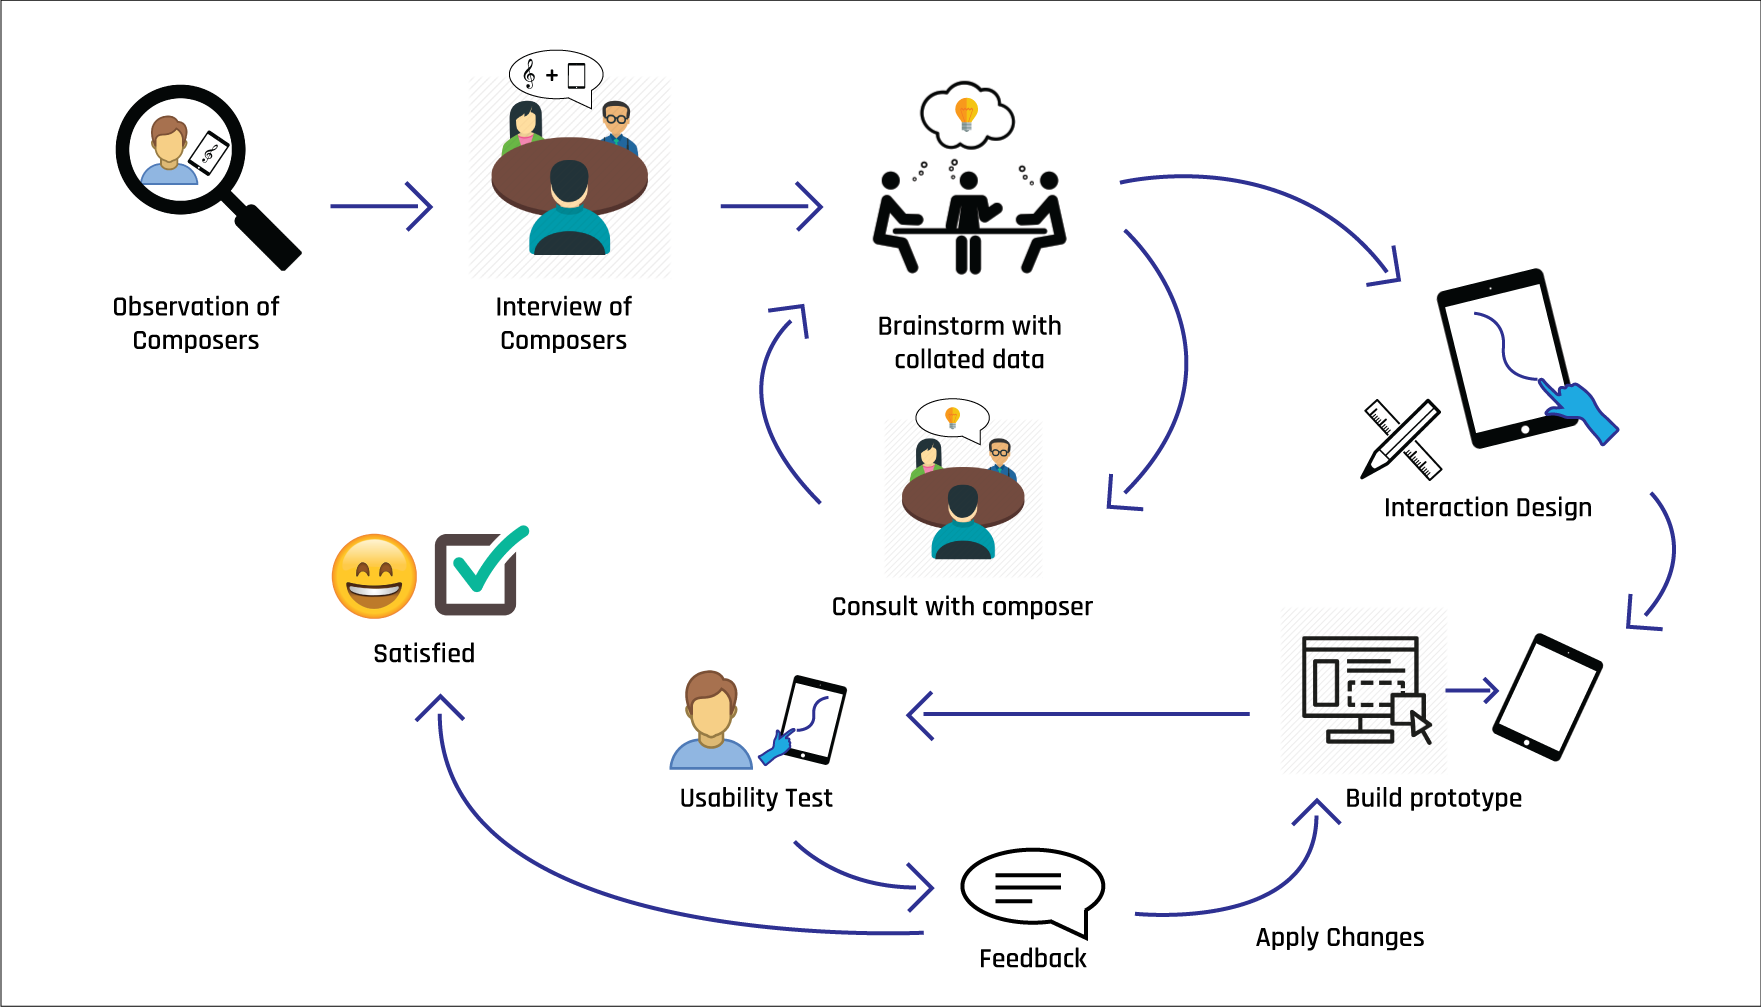
\includegraphics[scale=0.25]{Research_Framework}
    \caption{The research framework for Flow.}
    \label{fig:researchframework}
\end{figure}

This study was designed to be repetitive and iterative, to allow for continuous improvement of the system. User research and observation are important steps to understanding the behavior of users and figuring out their pain points. This is followed by interviews with composers to confirm and distill the information gathered from the research and observations. The points that were given by the composers would then be used in the brainstorming phase to determine a suitable solution. The team will then consult with the researchers about the proposed solution to gather their insights about it. The brainstorming would then be repeated to improve on the solution followed by another consultation. This would be repeated until the team is satisfied with the solution.

The next phase would involve designing the interaction of the proposed solution. This would be followed by the prototype phase where a prototype would be built, tested, and improved repeatedly. Usability tests would be performed with different prototypes to create a good user experience. This phase would be repeated multiple times until the researchers are satisfied with the results of the tests.

% \section{System Architecture and Framework}
\section{System Description}

\subsection{System Overview}

The system will integrate music theory and user experience in an interface for musical composition. The composition process of composers will be observed and analyzed so that the system can be built to fit this process. It will be built for the iOS, but will be optimized for the iPad. It will provide users an interface to create/edit, and view compositions. The user can interact with the system through a set of gestures that have been defined. Some gestures are intended for adding/editing/deleting notes while others are for musical metacreation. Finally, the system will allow users to save their composition, which would be saved using a MusicXML file unknown to the users.

\subsection{System Objectives}

	\subsubsection{General Objective}
		
        To provide an interface that allows composers to perform basic and advanced musical composition tasks via gesture interactions.

	\subsubsection{Specific Objectives}
    
    	Specifically, the system will allow users to do the following: 
          \begin{enumerate}
              \item View, create, edit, and delete their own compositions
              \item Play their compositions
              \item Set the clef, key signature, and time signature of their 								compositions
              \item Add, edit, and delete notes through tap and hold gestures
              \item Highlight a set of notes
              \item Play the highlighted set of notes
              \item View information on the pitch and octave of the notes
              \item Make a horizontal gesture to the right to generate a sequence of 						notes based on previous notes and coded rules
              \item Make a gesture to the right that goes up to generate a sequence of 						notes with an increasing pitch
              \item Make a gesture to the right that goes down to generate a sequence of 						notes with an decreasing pitch
              \item Make a swirling gesture to the right to generate a repeating 							sequence of notes
              \item While gesturing, decrease the generated gestures by going to the 						left
              \item Choose to confirm or cancel a sequence of notes generated by a 							gesture
              \item Save the composition to be stored in local storage    

          \end{enumerate}
    
\subsection{Scope and Limitations of the System}

Given that the system is on a mobile platform, it would be limited in ability compared to that of desktop applications. This system aims to be a sketching application for composers that are on the go, or do not have their computers available. It will not contend with full-blown desktop musical composition applications like Finale or Sibelius.

Musical composition can be done for several kinds of instruments. However, the way music is composed varies from one instrument to another. With that said, the system will only support compositions for the piano. The system will also limit the musical notation symbols that can be used. The ones available for use are: 

\begin{itemize}
	\item Sixty-fourth note to whole note
    \item Sixty-fourth rest to whole rest
    \item Accidentals (sharp, flat, double-sharp)
\end{itemize}

Composers will also need to save their compositions in cases where they could not finish entirely and want to go back to it. A composition also has several elements which would be hard to model in databases. Thus, MusicXML will be used as the file format for saving data. This also makes it easy to transfer work from the system to other musical composition applications.

Gesture interactions are the main method of interaction within the system. Some gestures like tapping on the line need to be accurate and precise. To improve this precision, bigger screens will be needed. The iPad will be the best for this due to it having a large screen, yet still being portable. The testing will also be done on the iPad only.

Finally, the system's musical metacreation will need to have a model for generating the succeeding notes. To make it lightweight, the system will make use of a rule-based model similar to that of Computoser \citep{bozhanov2014computoser} and SuperWillow \citep{schulze2011music}. The model will take into account music theory for its rules.

\subsection{Data Design}

Given that musical compositions have a lot of elements which need to be stored as data, using relational databases for storage would prove to be inefficient and unintuitive \citep{hristidis2003efficient}. That is why the system would represent data through the use of MusicXML, which was also used in the SuperWillow system found in the study of \citeauthor{schulze2011music}.

MusicXML is a method of storing and representing digital sheet music through XML \citep{makemusic2017musicxml}. Because it is an Extensible Markup Language (XML), it follows a specific format that defines a logical structure \citep{bray1997extensible}, which in this case is a musical composition. The advantage of the MusicXML format is that it is used in several musical composition applications and can easily be shared between these applications \citep{makemusic2017musicxml}. Also, it can represent the most complicated aspects of musical notation like repeats, slurs, and more.

Shown in Table \ref{tab:musicxml} are the some of the commonly used elements and their respective descriptions in MusicXML.
 
\begin{longtable}{|p{3.6cm}|p{10cm}|} 
\caption{Commonly Used MusicXML Elements} \label{tab:musicxml} \\
\hline
       
       Element & Description \\ \hline
		
        \texttt{<score-partwise>} & Defines that the composition is divided into several parts, and these parts can have multiple measures. \\ \hline
        
        \texttt{<score-timewise>} & An alternative to the \texttt{<score-timewise>}, it defines the composition to have multiple measures where the measures can have many parts. \\ \hline

		\texttt{<part-list>} & Lists the parts of the composition. \\ \hline
        
        \texttt{<score-part>} & To be used as a child of \texttt{<part-list>}, this element adds a new part to the composition. Commonly supplied with the \texttt{id} attribute. \\ \hline
        
        \texttt{<part-name>} & A child of the \texttt{<score-part>} element, specifies the name of its parent part. \\ \hline
        
        \texttt{<attributes>} & Lists essential information in the composition such as the key, time signature, and clef. \\ \hline
        
        \texttt{<divisions>} &  Used in the production of sound. It works with the \texttt{<duration>} element to tell how many divisions per quarter note equal to the duration indicated. \\ \hline
        
        \texttt{<key>} & Denotes which key signature the composition is in and contains the \texttt{<fifths>} element. \\ \hline
        
        \texttt{<fifths>} & This element is derived from the circle of fifths and says how many sharps or flats the composition has. \\ \hline
        
        \texttt{<time>} & The time element contains information about the time signature which can be set using the \texttt{<beats>} and \texttt{<beat-type>} tags. \\ \hline
        
        \texttt{<beats>} & The numerator of the time signature. \\ \hline
        
        \texttt{<beat-type>} & The denominator of the time signature. \\ \hline
        
        \texttt{<clef>} & Tells the clef to be used in the composition through the \texttt{<sign>} and \texttt{<line>} tags. \\ \hline
        
        \texttt{<sign>} & Specifies the sign to be used for the clef.\\ \hline
        
        \texttt{<line>} & Specifies which line the set sign will start. \\ \hline
        
        \texttt{<note>} & Contains information inside that is needed to define a single note. \\ \hline
        
        \texttt{<pitch>} & Located inside the \texttt{<note>} element, it contains the \texttt{<step>} and \texttt{<octave>} elements that would indicate where the note would be placed. \\ \hline
        
        \texttt{<step>} & Indicates the pitch step. Must always be supplied in the \texttt{<pitch>} element. \\ \hline
        
        \texttt{<octave>} & Indicates the octave of the pitch. Also required. \\ \hline

        \texttt{<alter>} & An optional element in the \texttt{<pitch>} that indicates if the note has a sharp or flat. \\ \hline
        
        \texttt{<duration>} & Also an element inside the \texttt{<note>}, it works with the \texttt{<division>} element to denote what kind of note or sound it would play. \\ \hline
        
        \texttt{<type>} & Mainly serves to indicate how the note will be displayed or notated. \\ \hline


\end{longtable}

Whenever a user creates a composition and saves it in the application, a corresponding MusicXML will be generated and saved in the device's local storage. The MusicXML will be used to load the composition again, in case the user wants to edit or view it. 

\subsection{System Framework}

\begin{figure}[H]
	\centering
	
\includegraphics[scale=0.4]{System_Framework}
    \caption{The system framework for Flow.}
    \label{fig:systemframework}
\end{figure}

The system framework, shown in Figure \ref{fig:systemframework}, illustrates an overview of how Flow works. Input is relatively simple, mainly in the form of gestures. Users can tap, swipe, hold, or drag on specific objects. The application's gesture recognizer would then analyze the gesture performed by the user. The system would then output or perform the specific action assigned to each gesture. However, if the gesture is tied to musical metacreation, the application would output a set of notes based on its built-in algorithm.

\subsection{System Walkthrough}

\begin{enumerate}

\item Start Menu - The user may create a new composition or edit existing ones on this screen. After opening a composition or creating a new one, the editor screen will be shown.

\begin{figure}[H]
	\centering
	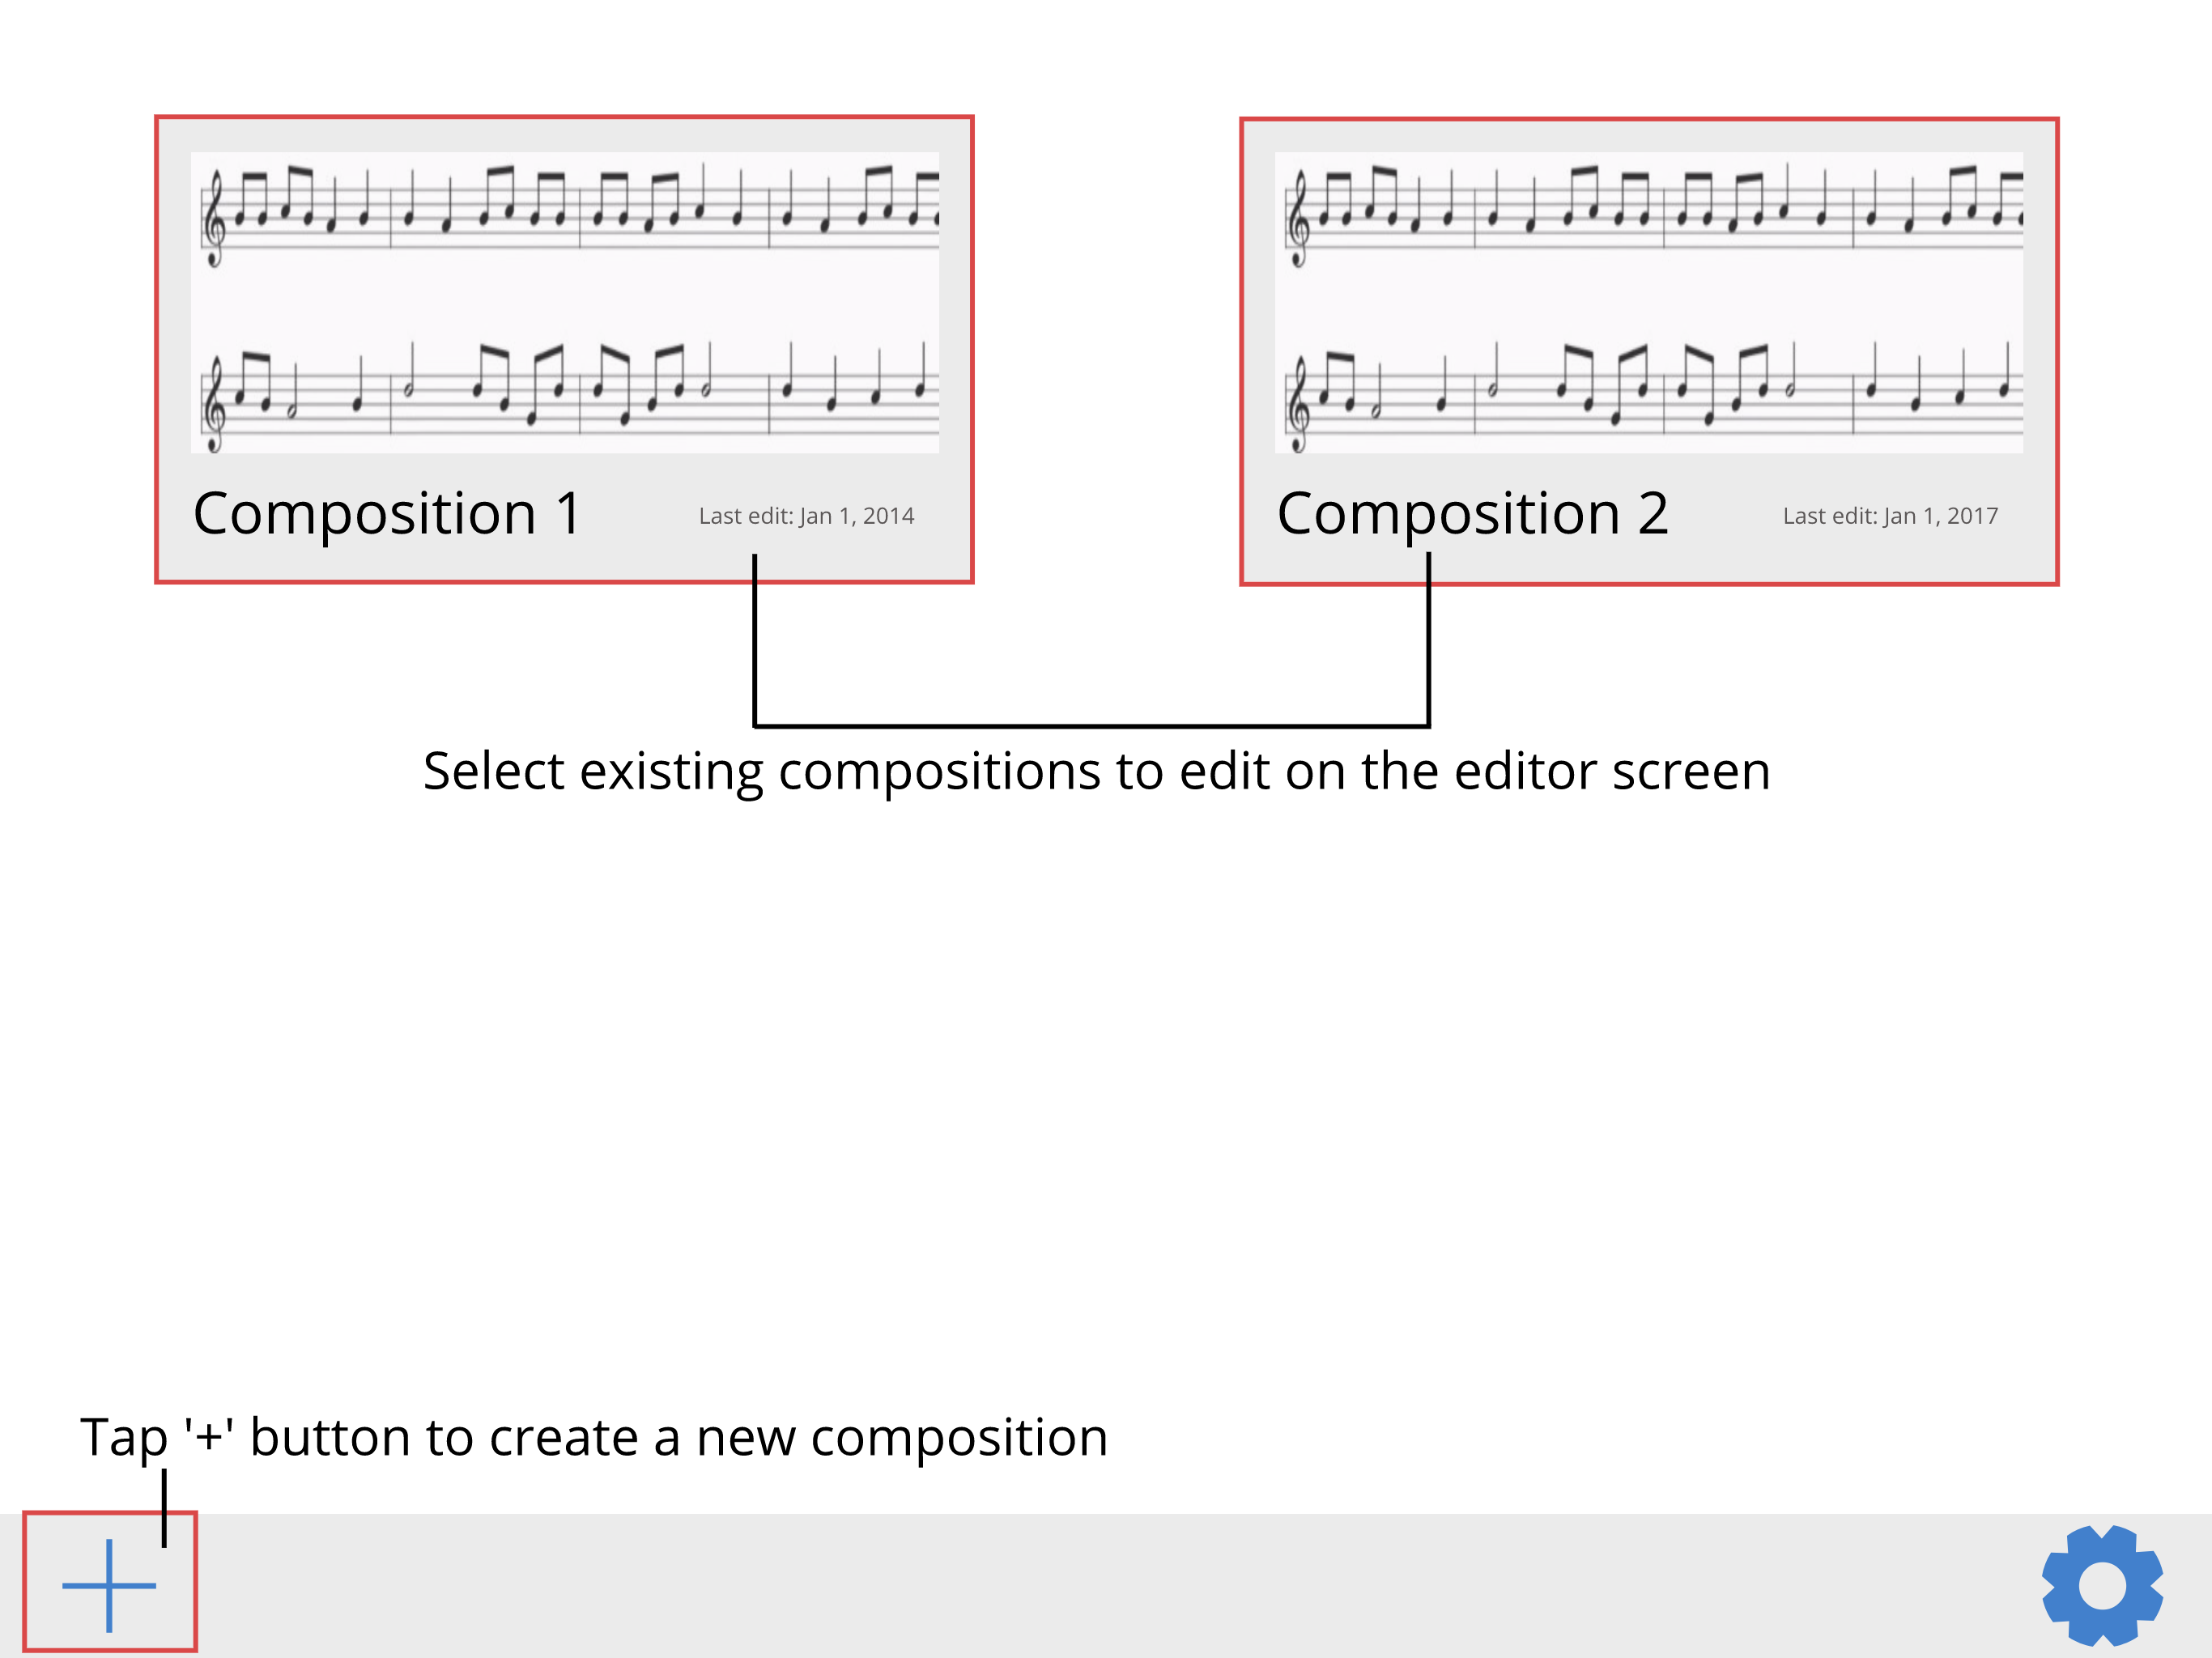
\includegraphics[scale=0.28]{Start_Menu}
    \label{fig:startmenu}
    \caption{Start menu screen.}
\end{figure}

\item Editor - The user may start creating a composition on this screen. The user may add, edit, delete, copy, cut, or paste notes using the menu. The user may also generate music using the gesture space and set or edit the time signature.

\begin{figure}[H]
	\centering
	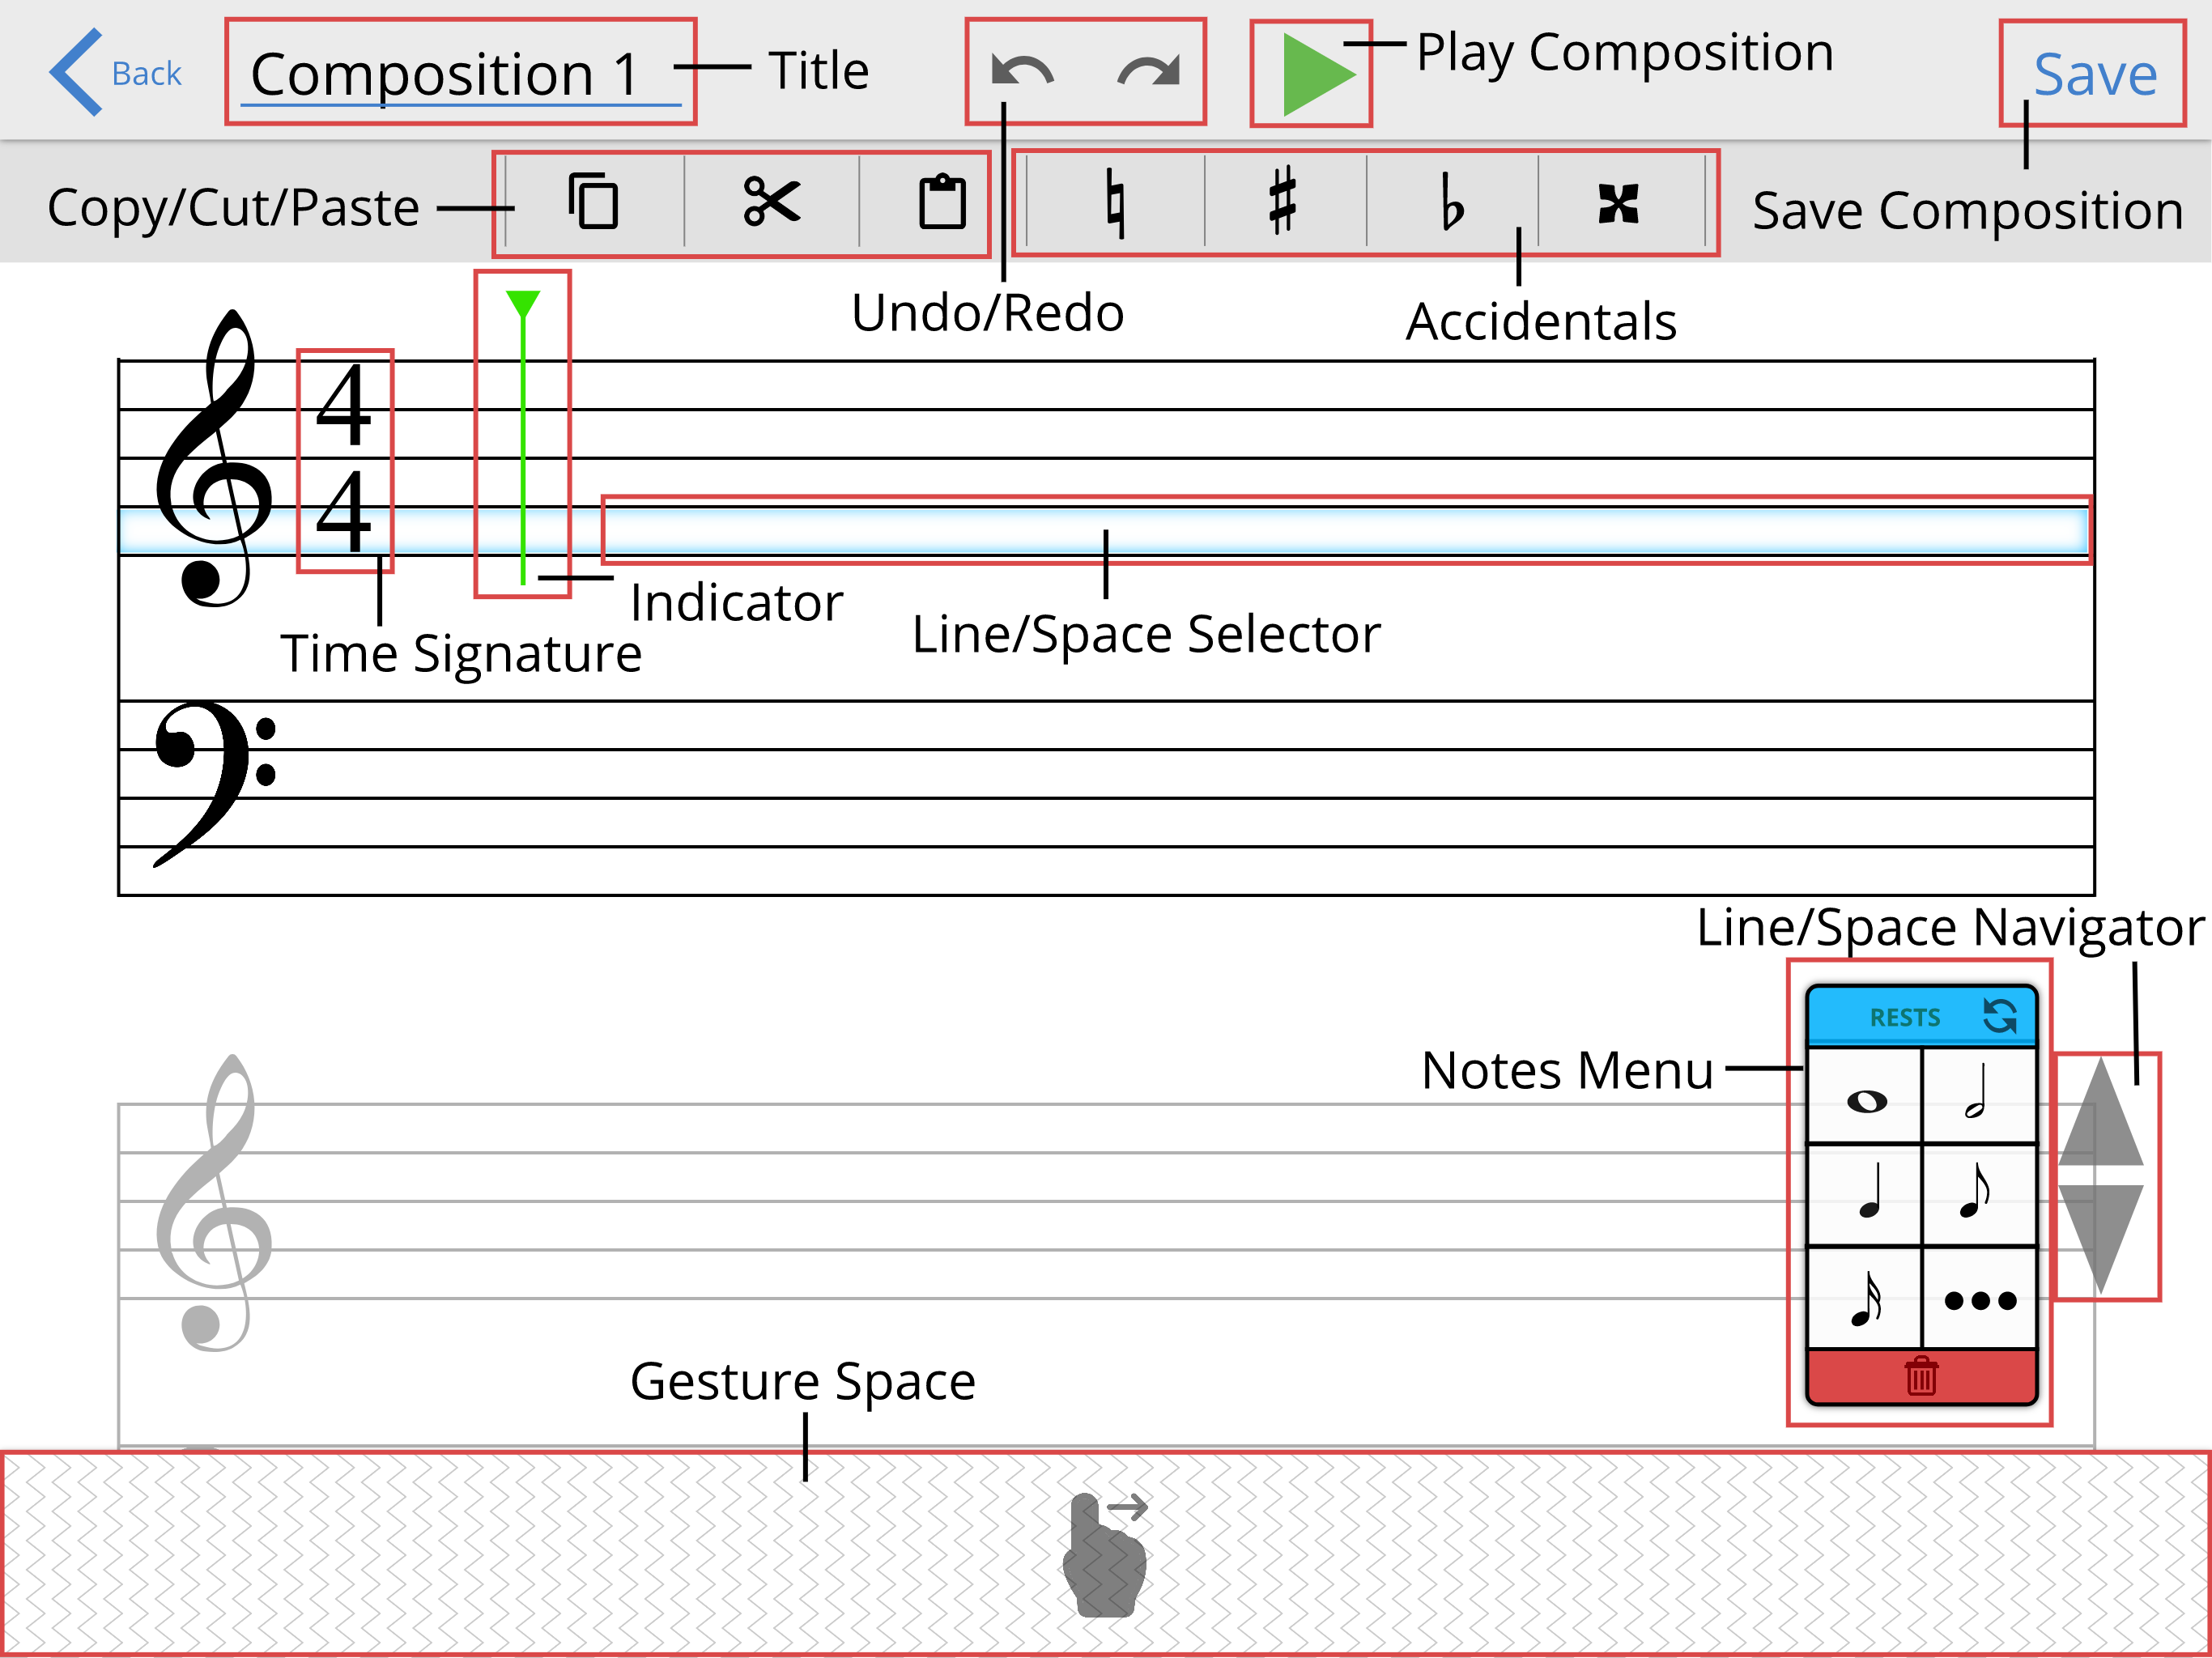
\includegraphics[scale=0.28]{Editor}
    \label{fig:editor}
    \caption{Editor screen.}
\end{figure}

\item Selecting a Note

To select a note, tap on a note on the staff.

\begin{figure}[H]
	\centering
	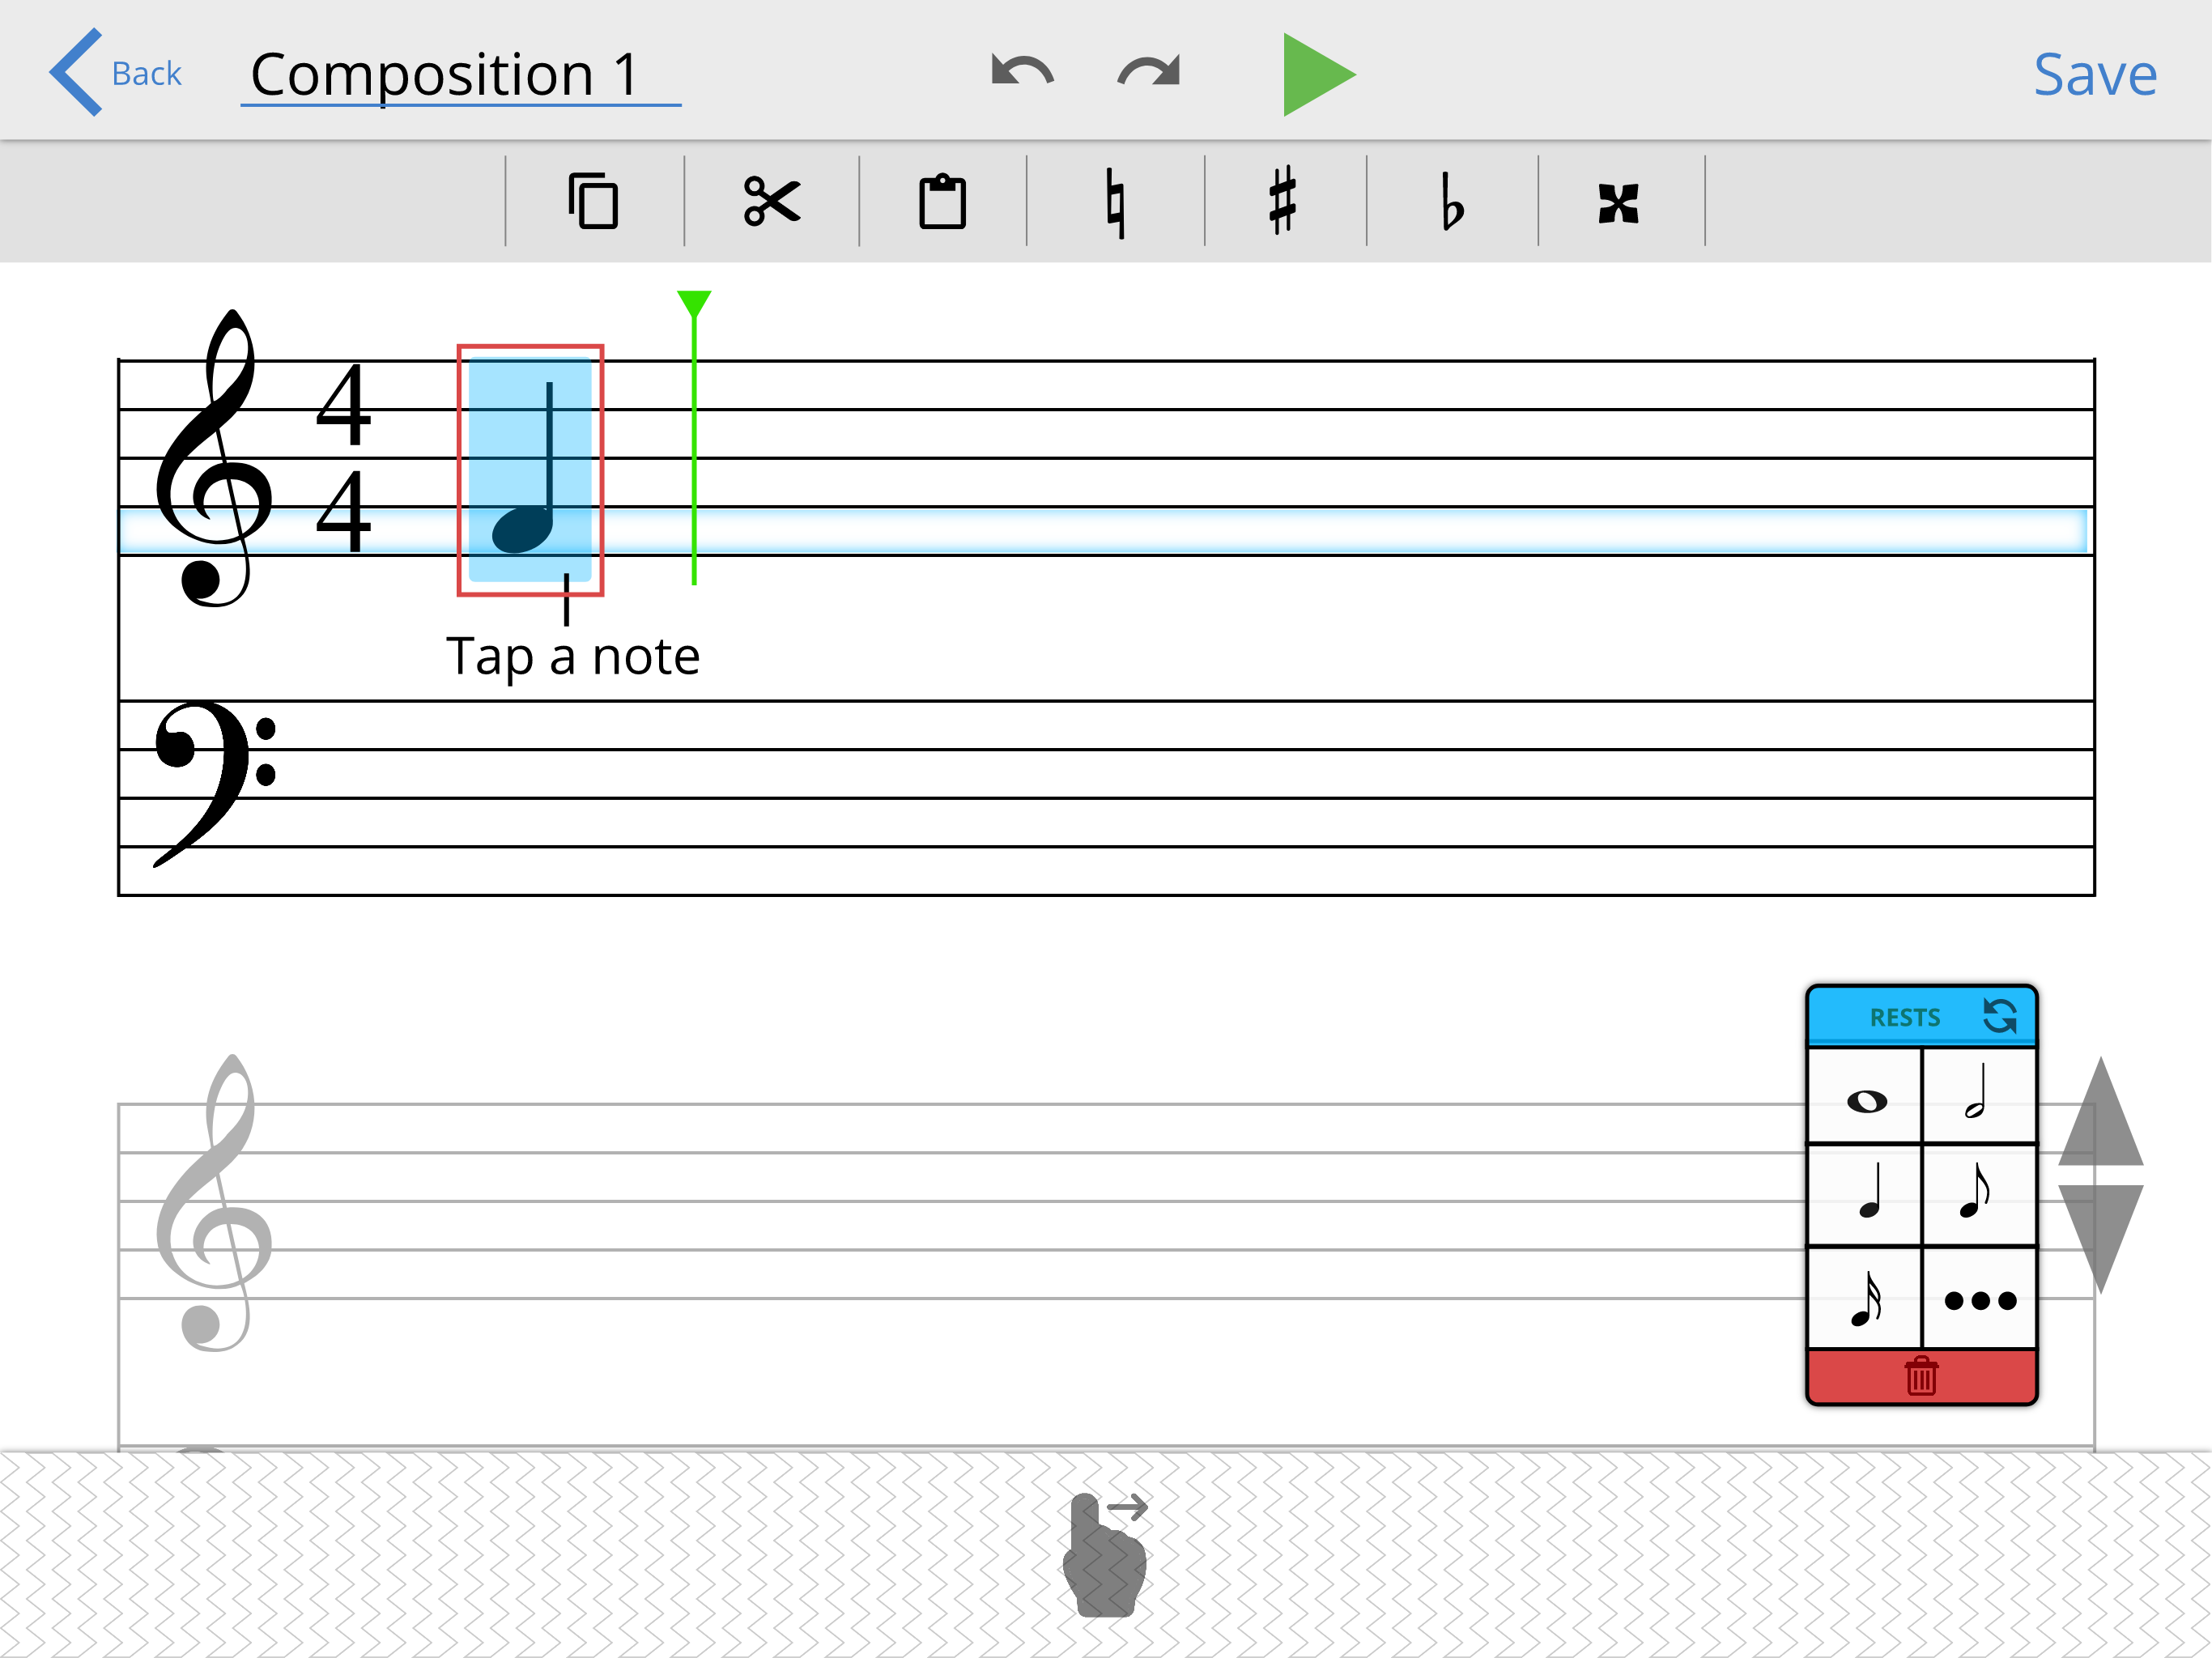
\includegraphics[scale=0.28]{Selecting_a_Note}
    \label{fig:select-note}
    \caption{Tap on a note to select it.}
\end{figure}

\item Selecting Notes

To select multiple notes, drag diagonally upward or downward on the notes.

\begin{figure}[H]
	\centering
	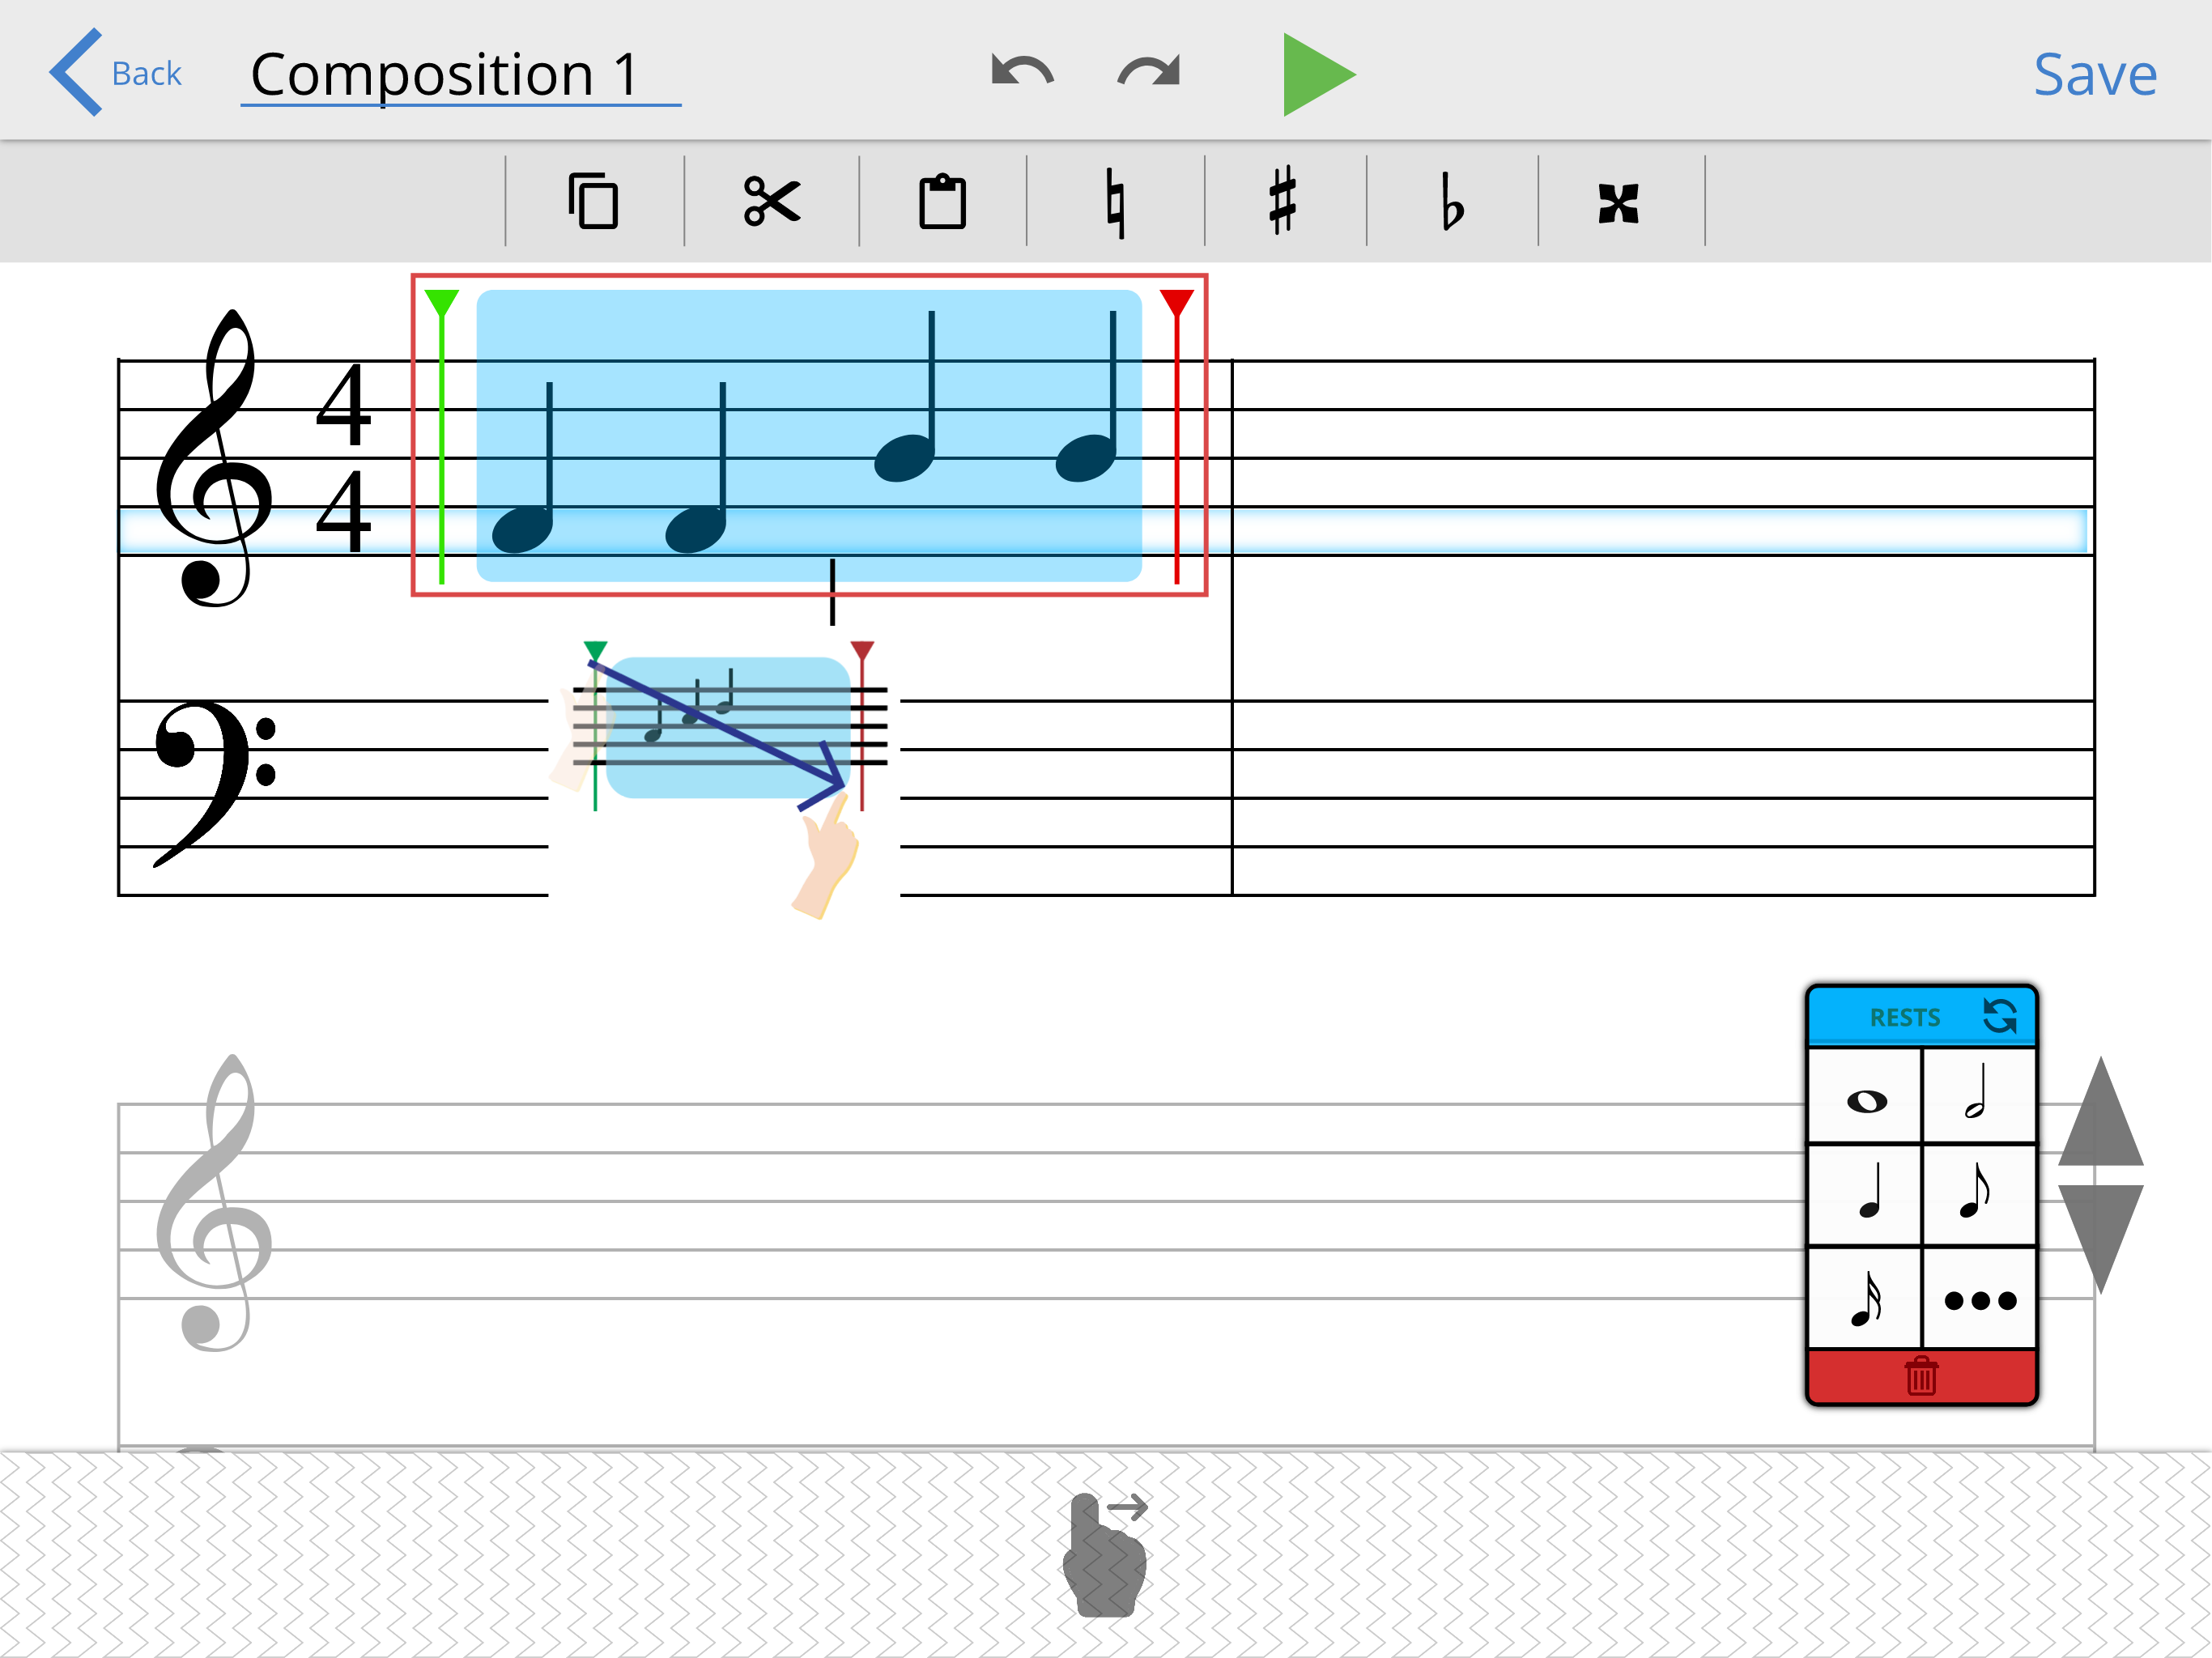
\includegraphics[scale=0.28]{Selecting_Notes}
    \label{fig:select-notes}
    \caption{Drag diagonally to select multiple notes.}
\end{figure}

\item Changing Time Signature and Key Signature

To change the time signature of a composition, tap on the time signature and a menu will pop up.

Slide the number of beats and/or the beat duration to change the number.

Tap key signature to change.

Tap save button to save changes.

\begin{figure}[H]
	\centering
	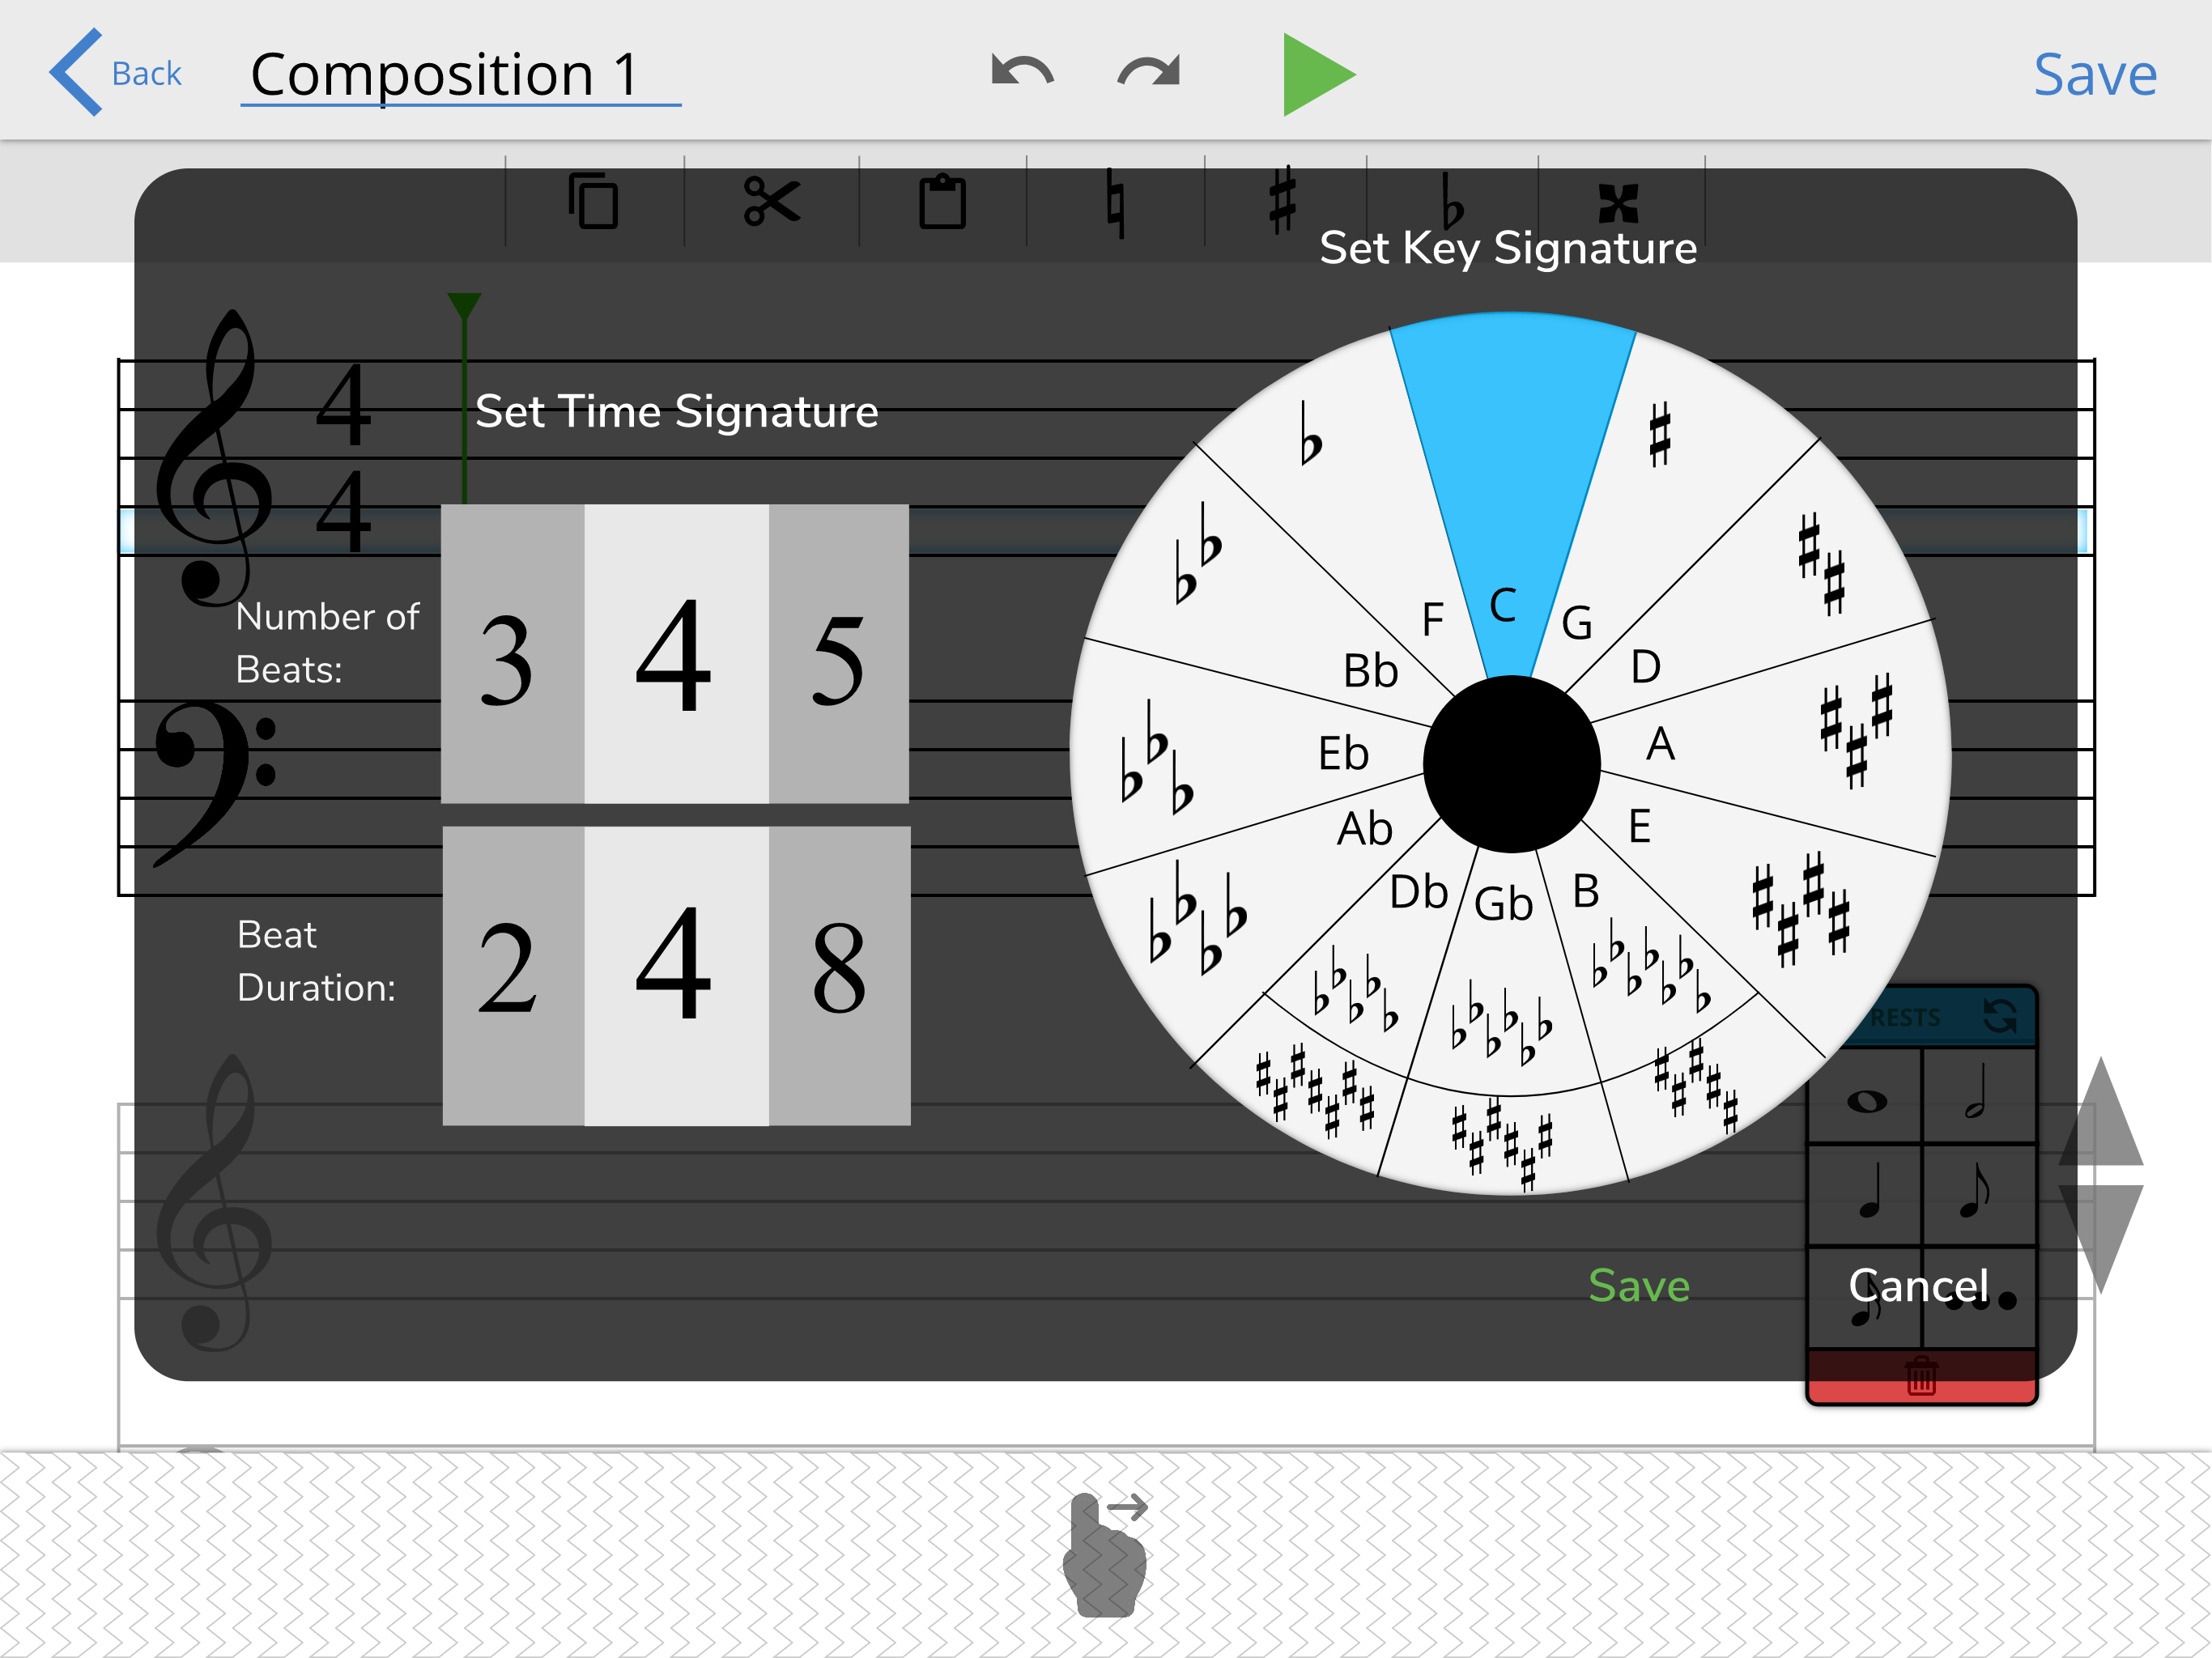
\includegraphics[scale=0.28]{Changing_Time_Signature}
    \label{fig:changetimesig}
    \caption{Slide the number of beats or beat duration to change the number.}
\end{figure}

\item Adding Notes

To add a note, tap on a preferred note in the menu and the note will be automatically placed on the location of the green indicator on the staff with the highlighted space or line.

\begin{figure}[H]
	\centering
	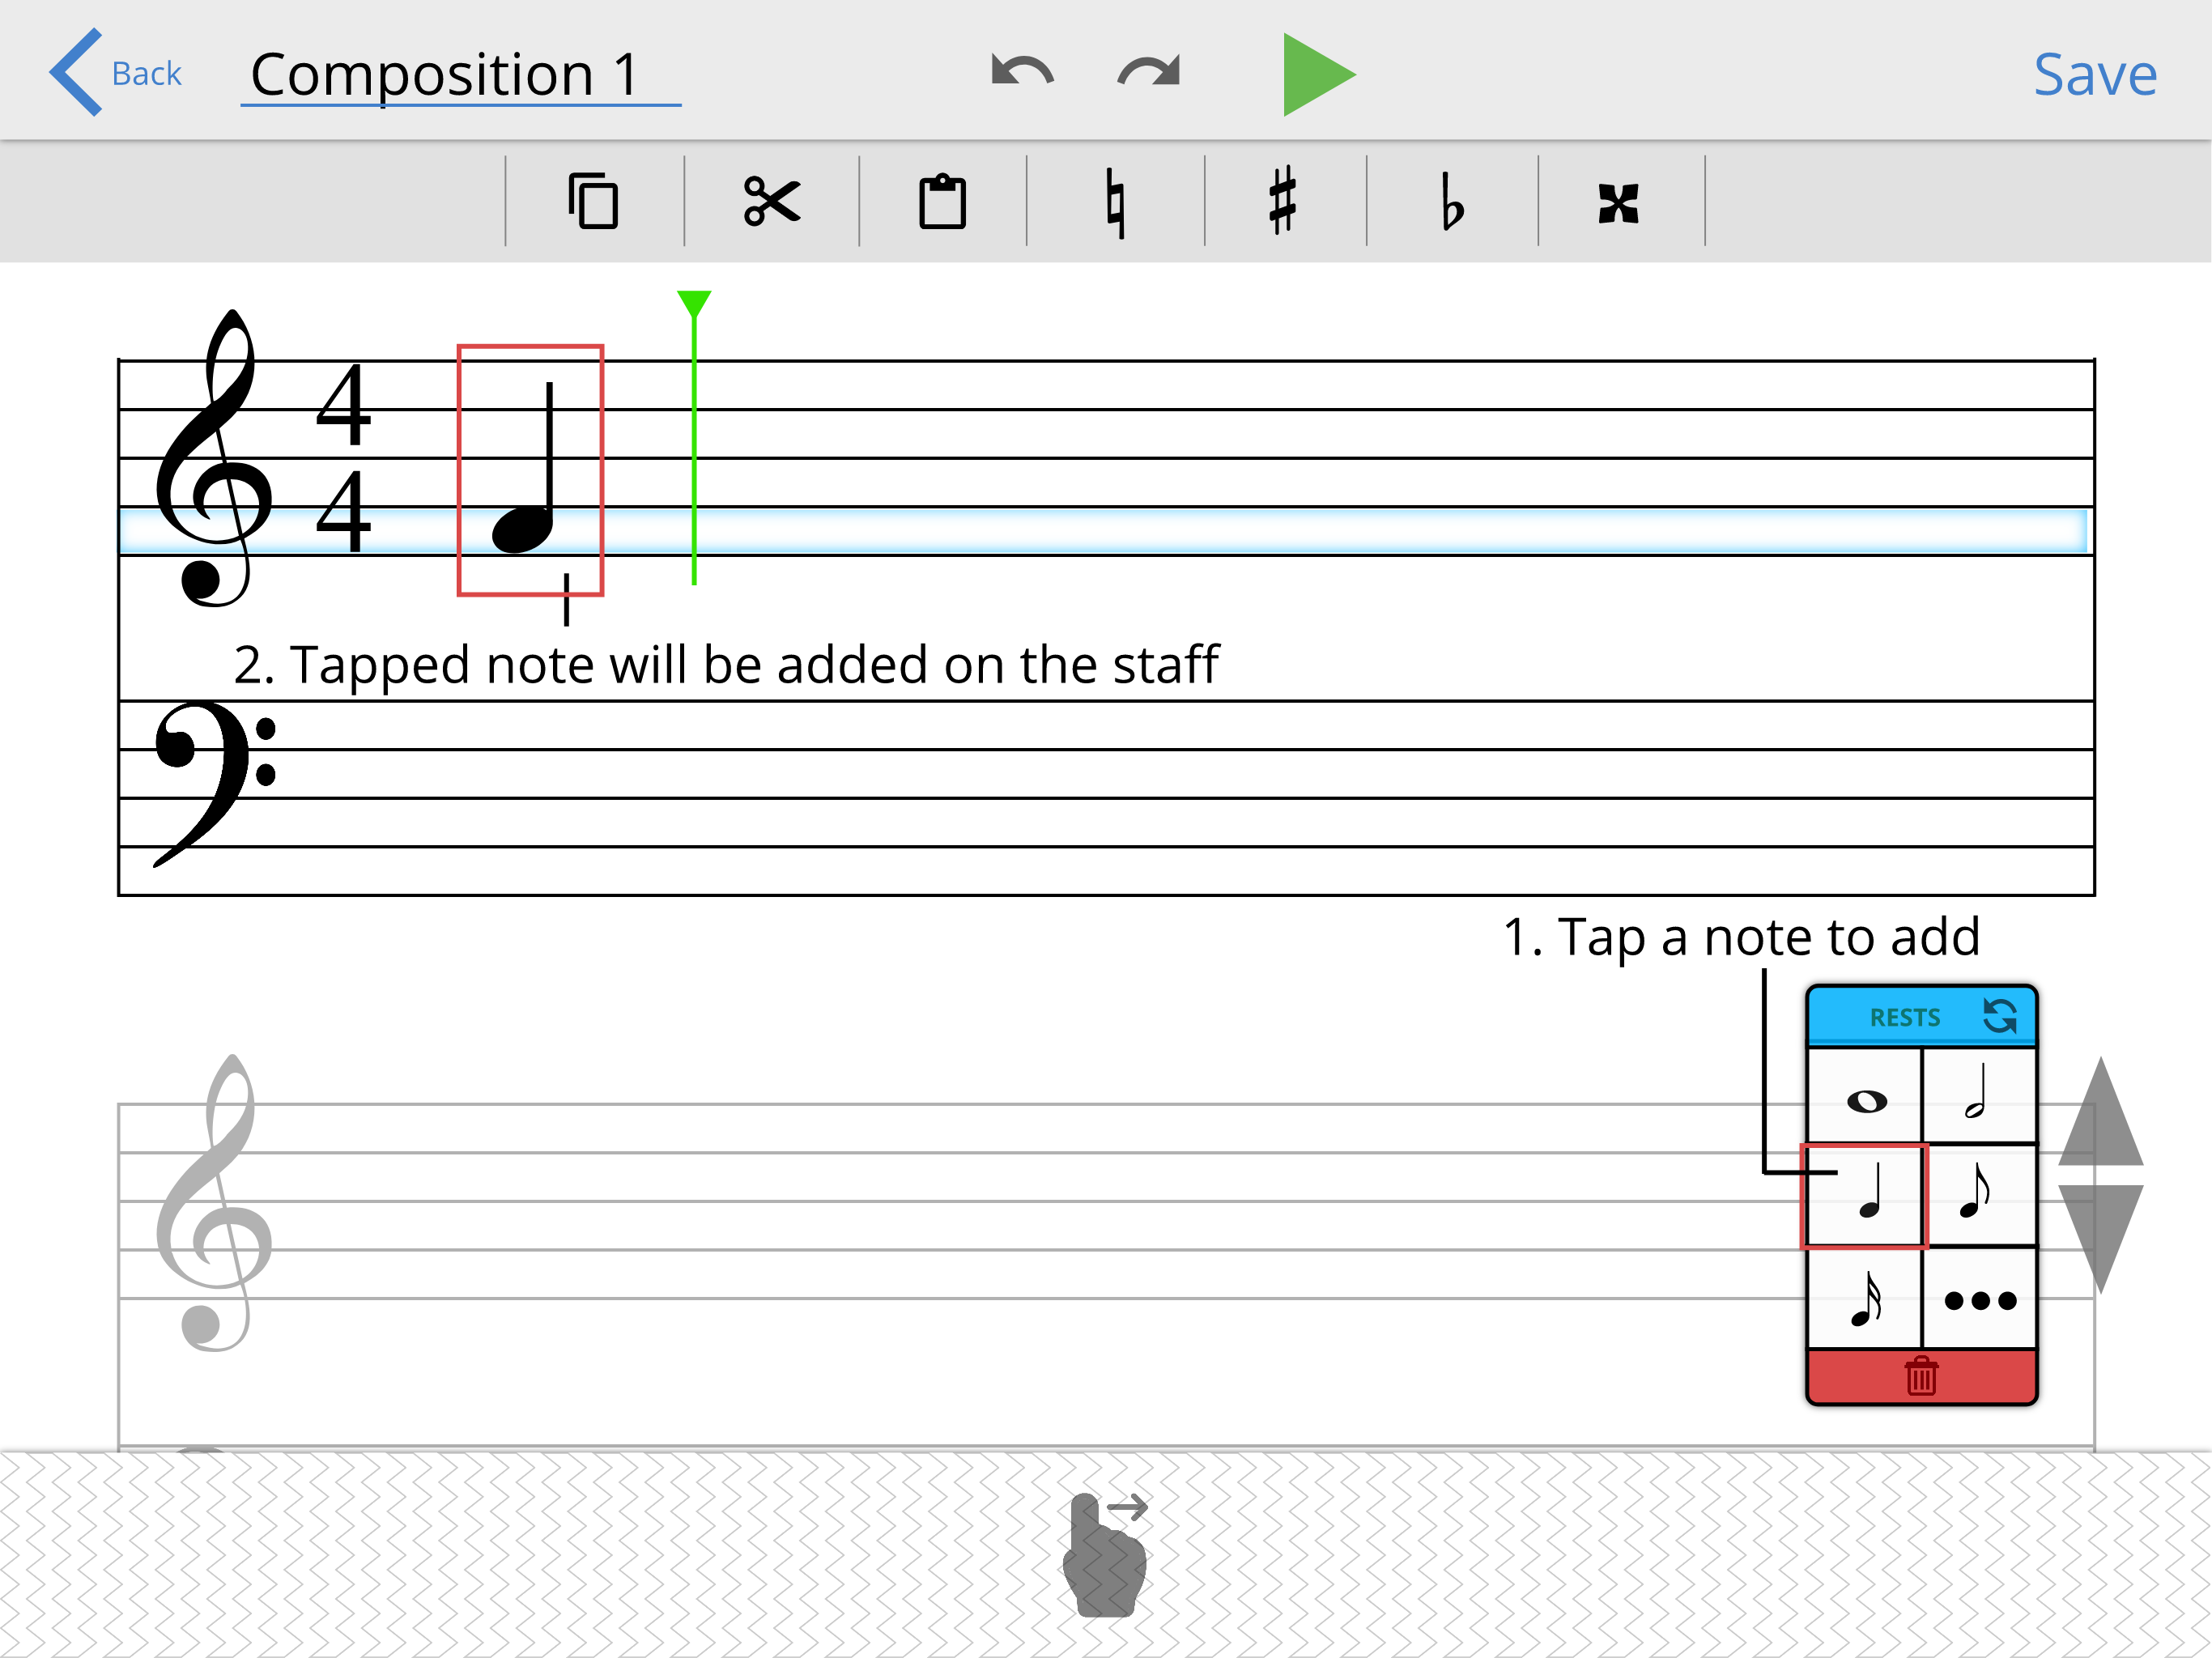
\includegraphics[scale=0.28]{Adding_Notes}
    \label{fig:add-note}
    \caption{Tap a note on the menu to add on the staff.}
\end{figure}

\item Adding Accidentals

To add an accidental, choose an accidental by tapping on the menu.

Add a note and the accidental will be added with it.

\begin{figure}[H]
	\centering
	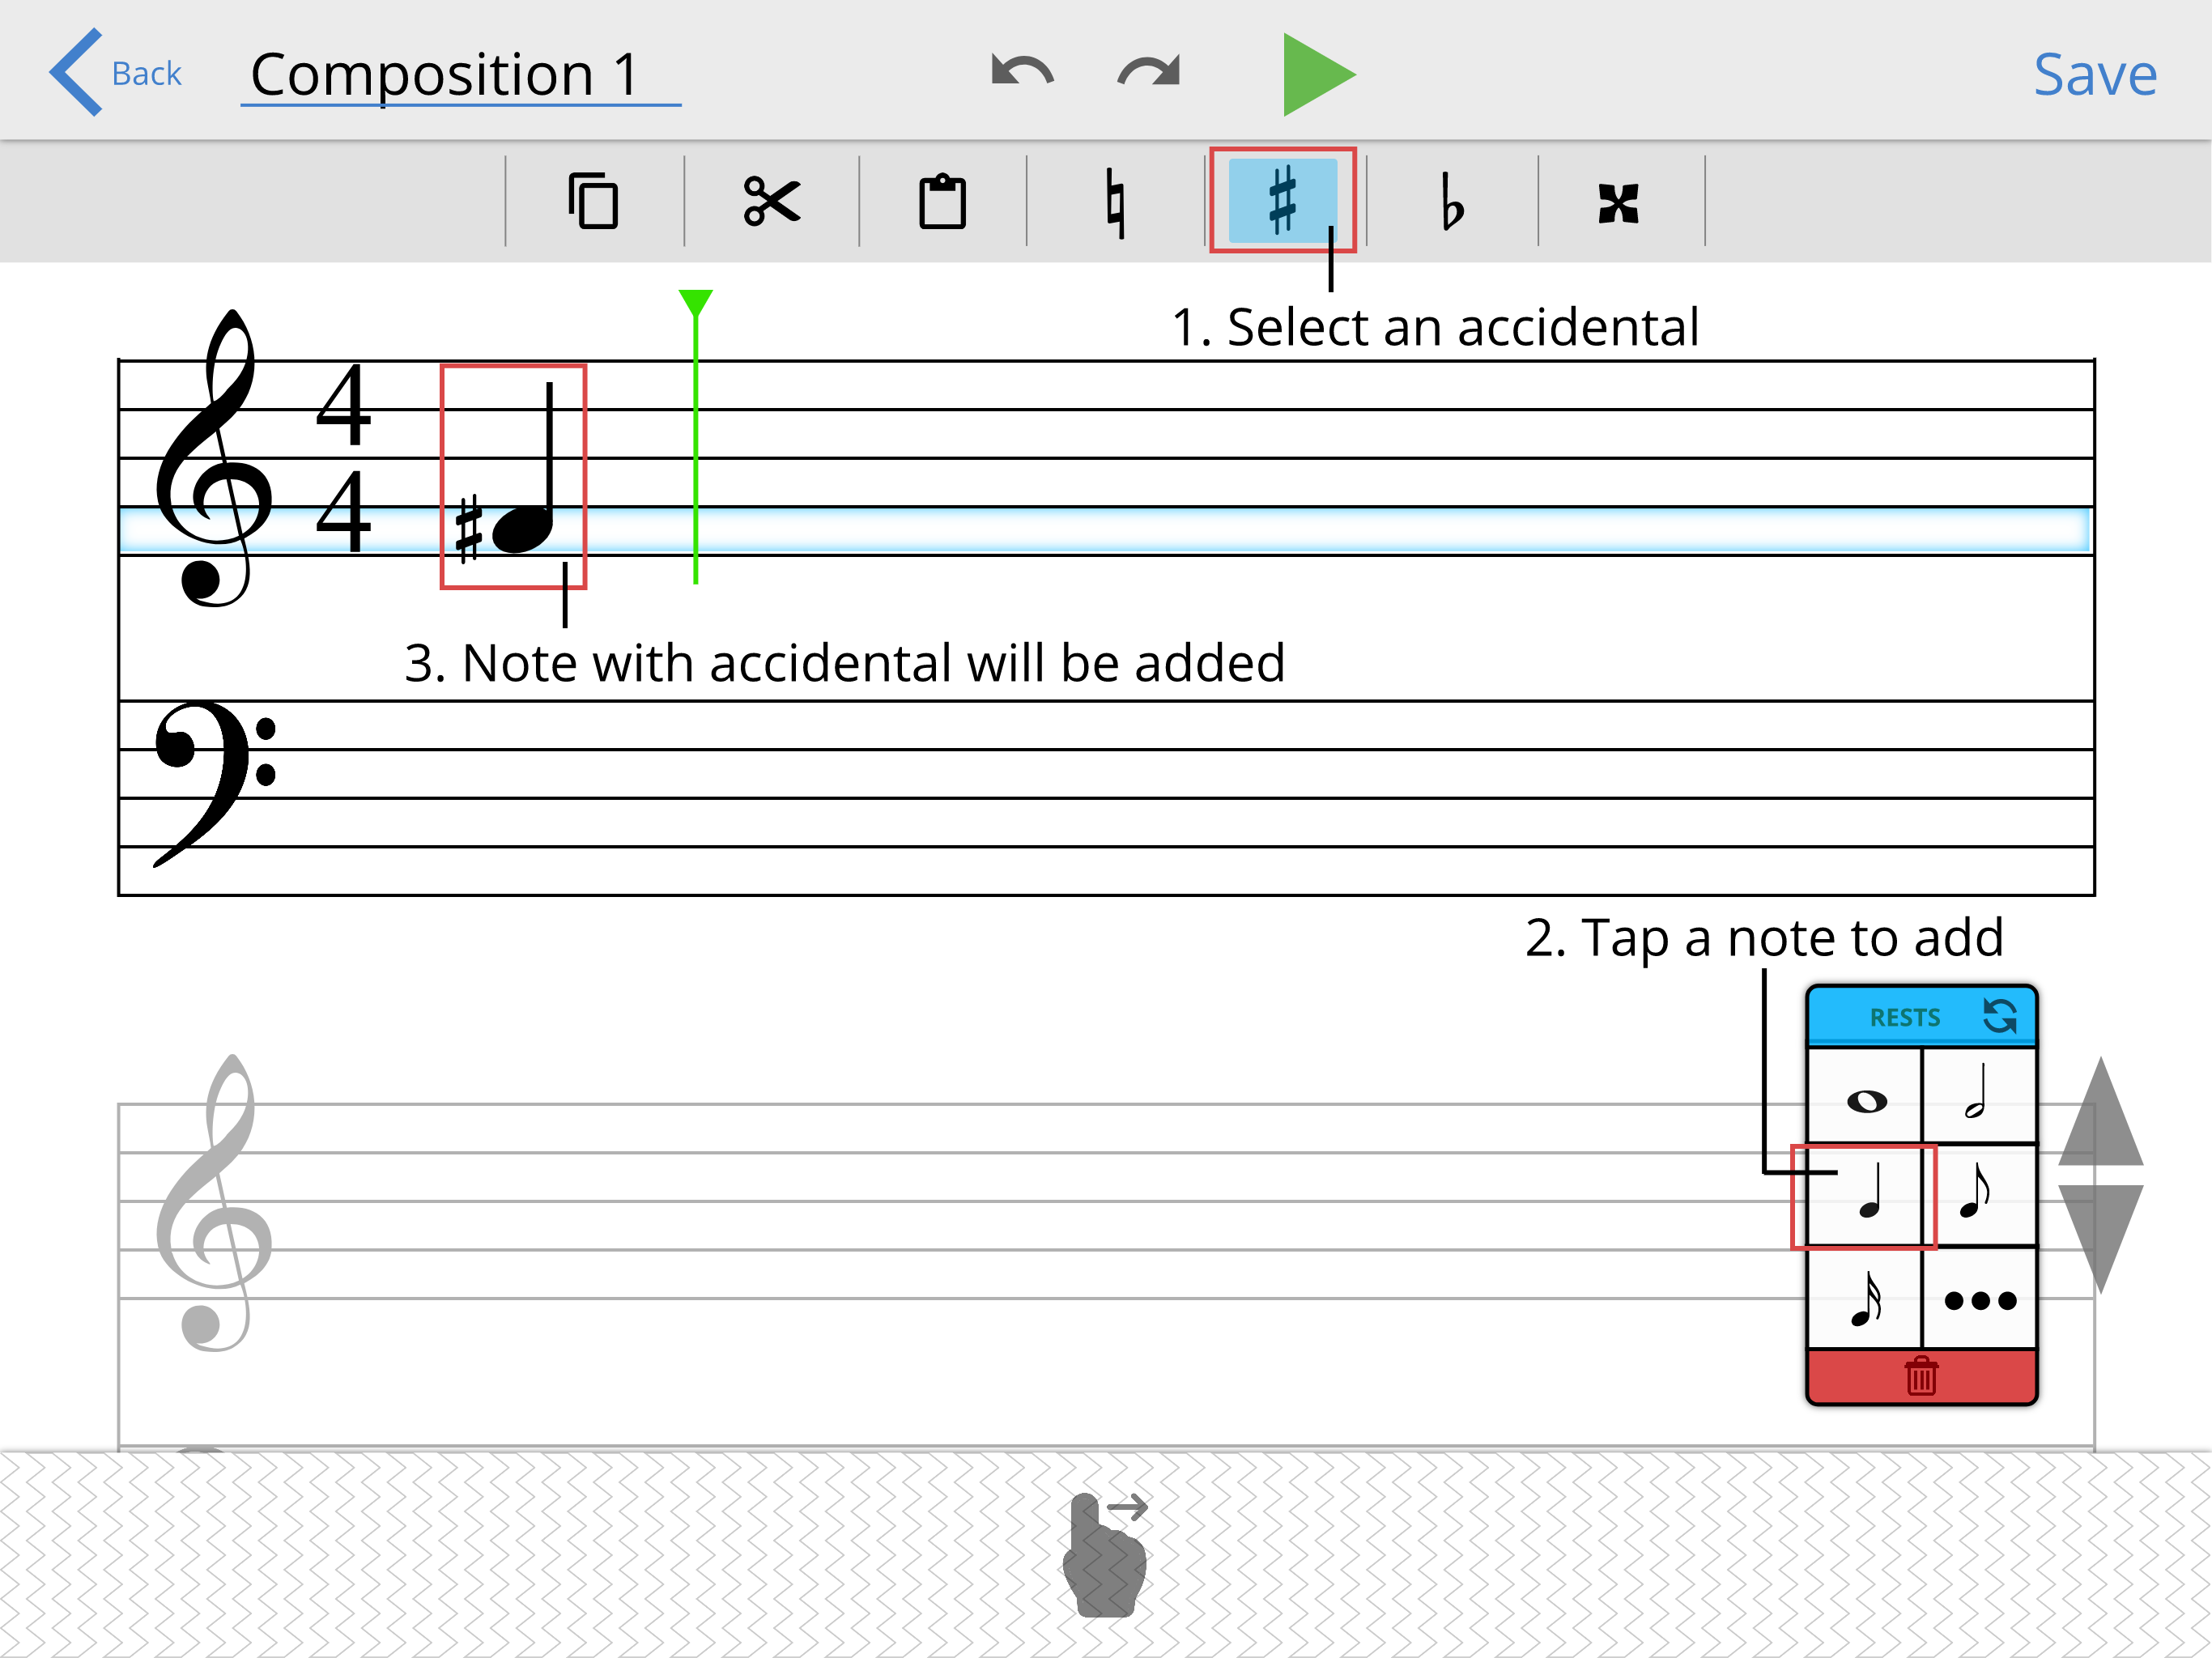
\includegraphics[scale=0.28]{Adding_Accidental}
    \label{fig:add-accidental}
    \caption{Tap an accidental on the menu and add a note.}
\end{figure}

\item Editing Notes

To edit a note, tap a note to select it, then click on the desired note on the menu.

\begin{figure}[H]
	\centering
	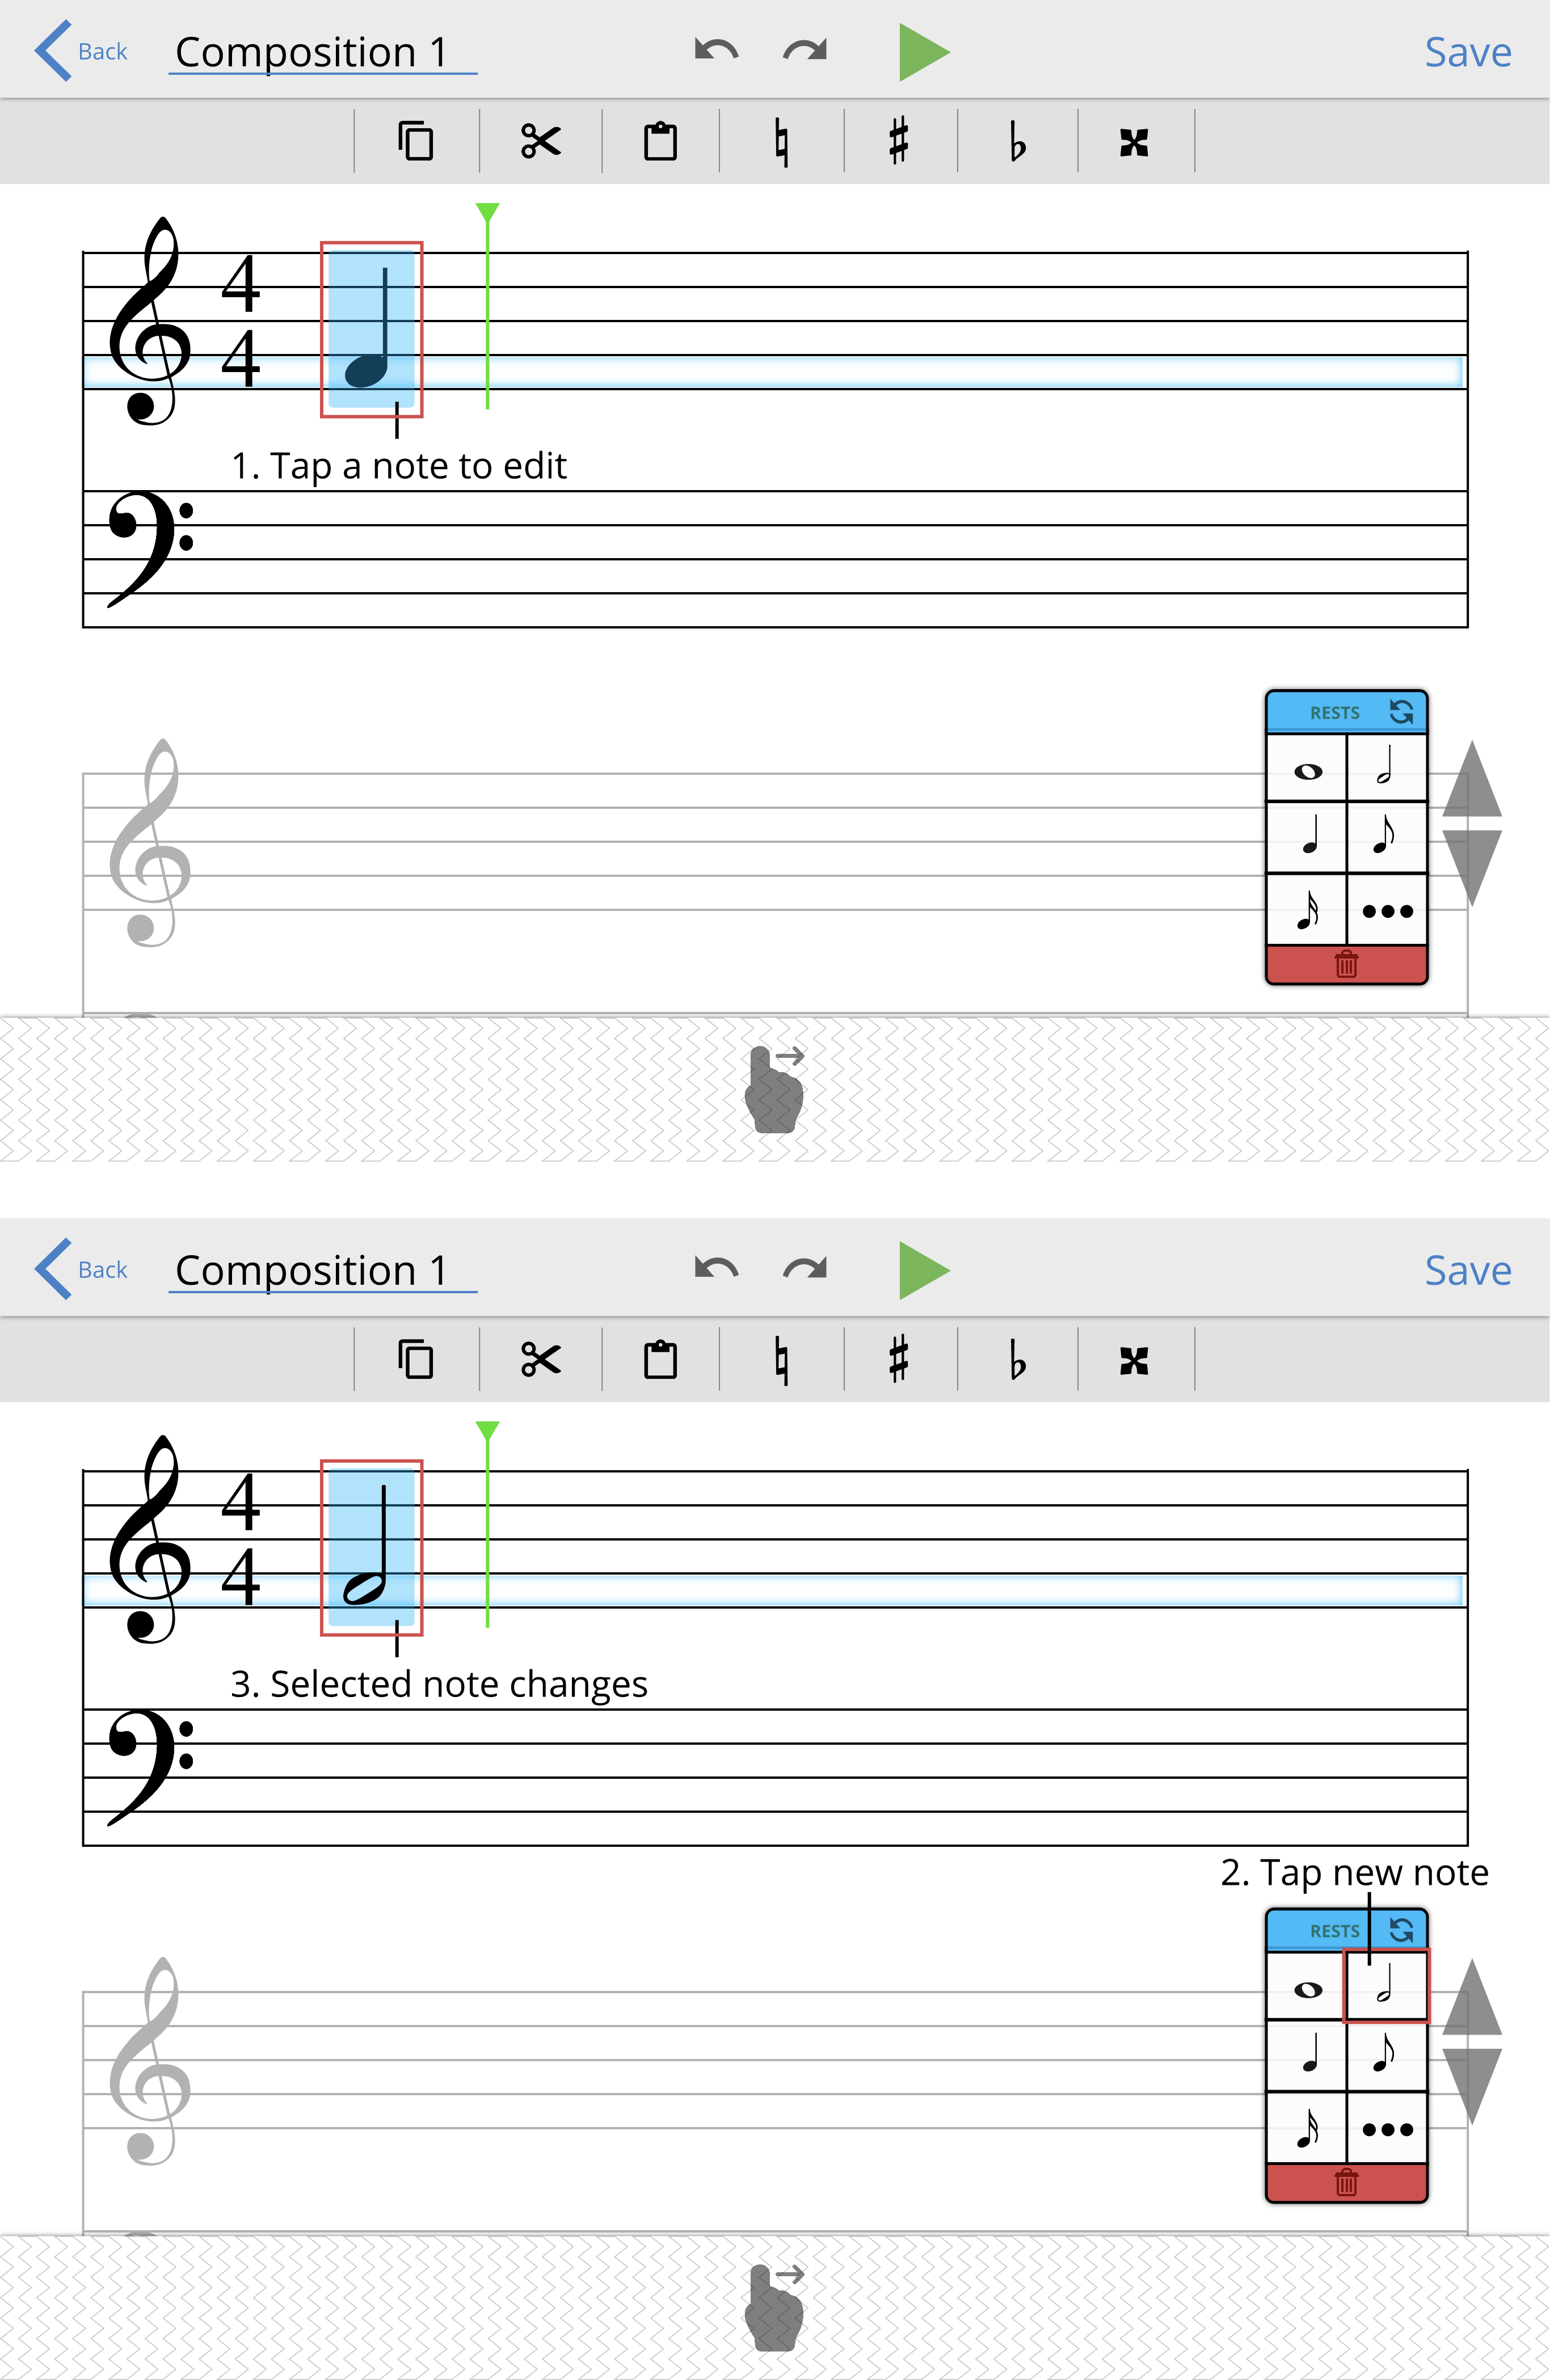
\includegraphics[scale=0.28]{Editing_Notes}
    \label{fig:edit-notes}
    \caption{Edit note/s by tapping the desired note on the menu.}
\end{figure}

\item Copy/Cut/Pasting Notes

To copy or cut a note or a set of notes, tap a note or highlight a set of notes on the staff to select, then tap the copy or cut button on the menu below the composition title to copy. Tap the paste button to paste the notes.

\begin{figure}[H]
	\centering
	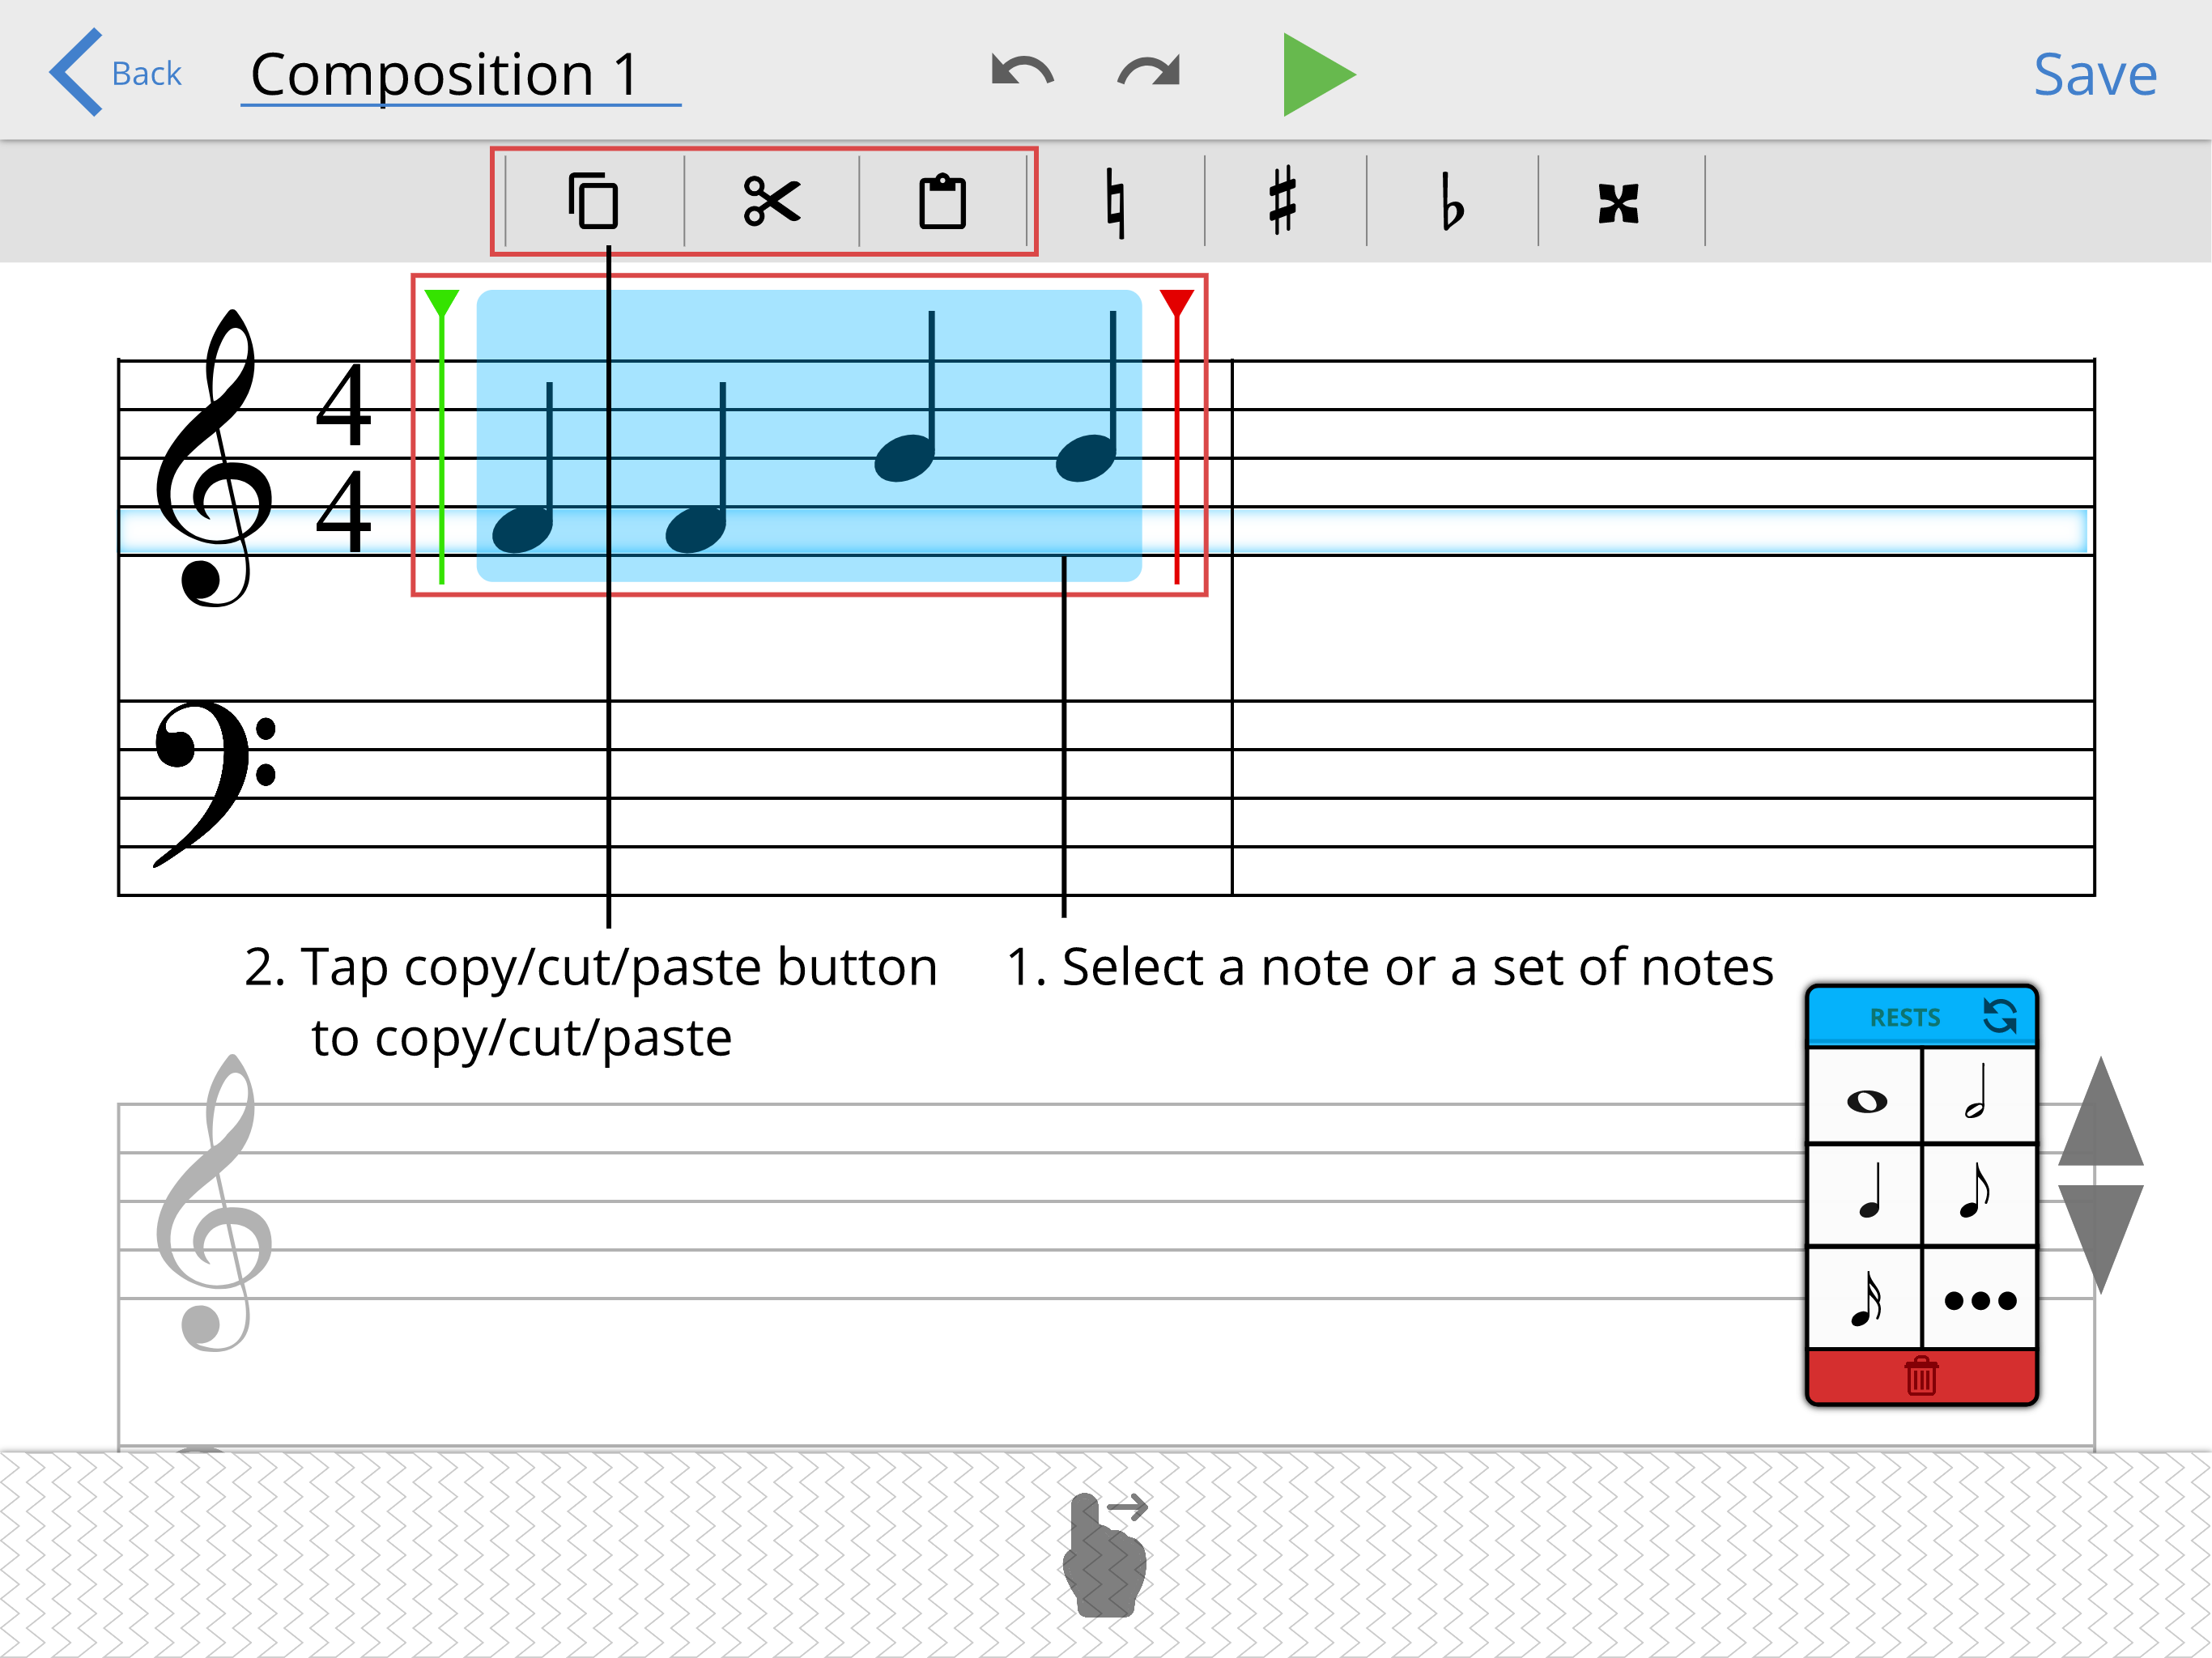
\includegraphics[scale=0.28]{Copying_Notes}
    \label{fig:copynotes}
    \caption{Copy or cut note/s by selecting note/s and then tapping copy/cut button. Tap paste to paste notes.}
\end{figure}

\item Deleting Notes

To delete a note or a set of notes, tap a note or highlight a set of notes on the staff to select, then make a two-finger flick gesture on the selected note/s or tap the delete button on the menu.

\begin{figure}[H]
	\centering
	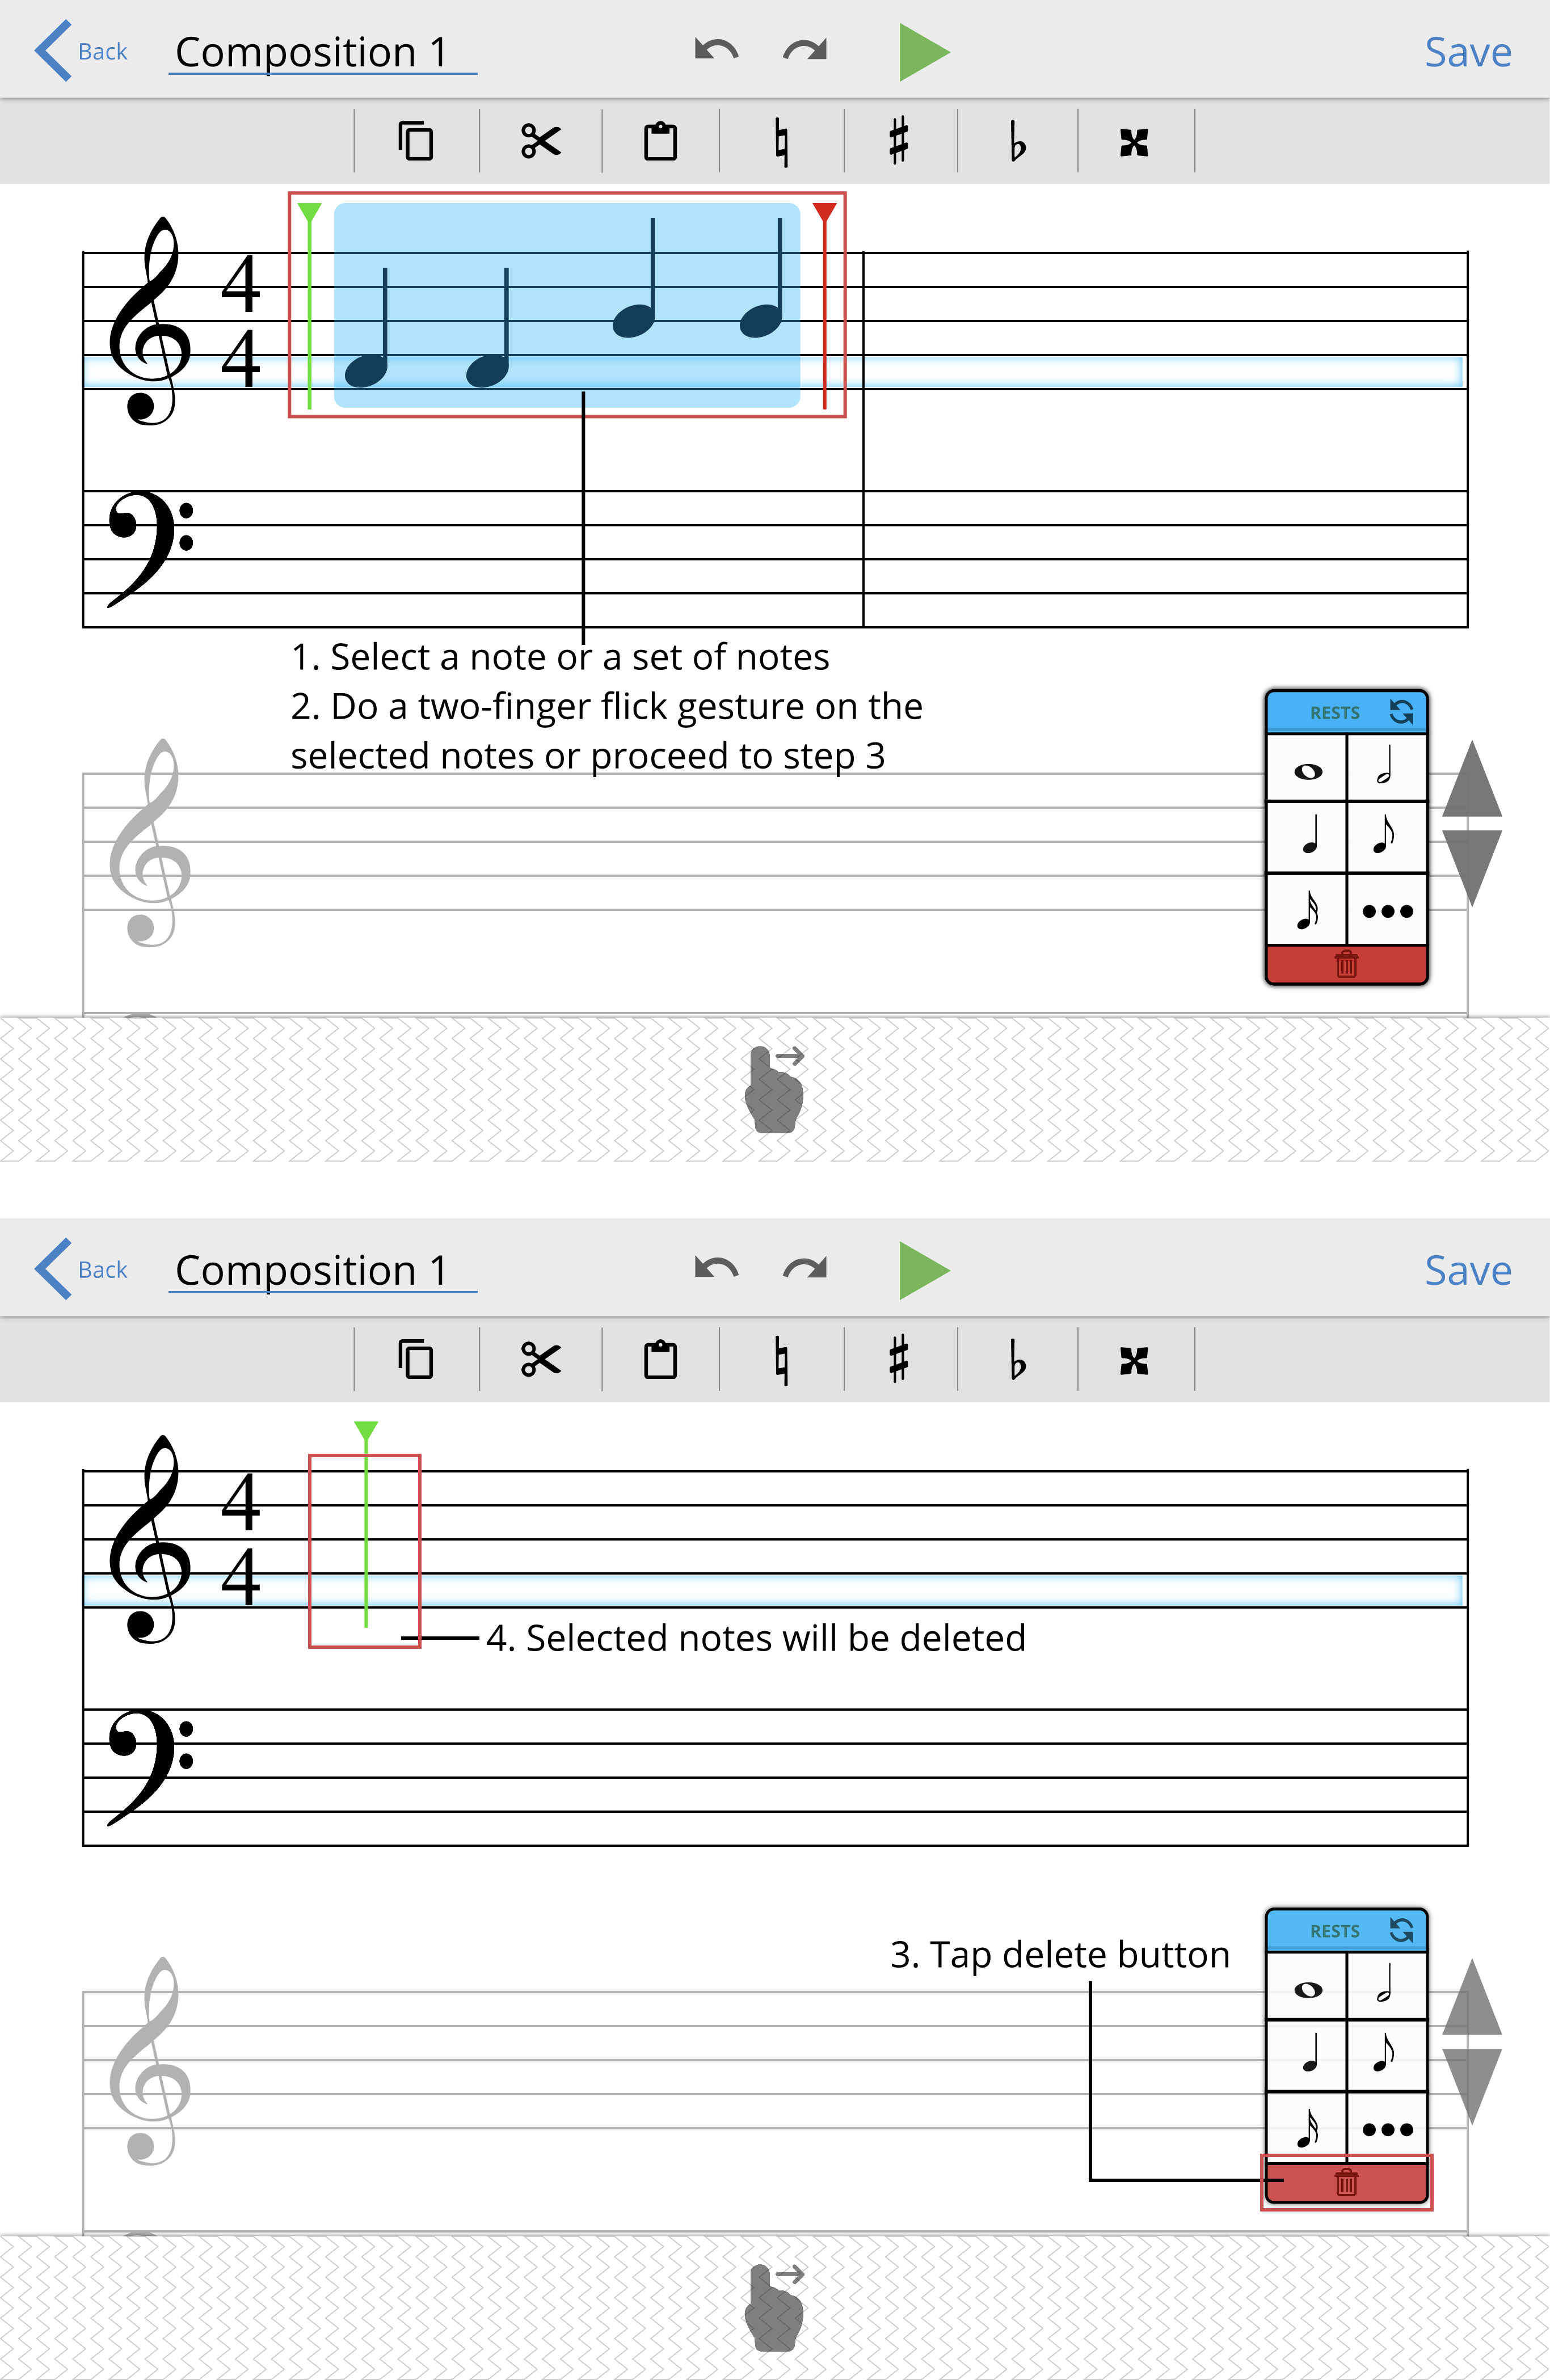
\includegraphics[scale=0.28]{Deleting_Notes}
    \label{fig:delete-notes}
    \caption{Delete note/s by tapping delete on the menu or by making a flick gesture on the selected note/s.}
\end{figure}

\item Transposing Notes

To transpose selected notes, make a two-finger swipe up or down gesture on the gesture space.

\begin{figure}[H]
	\centering
	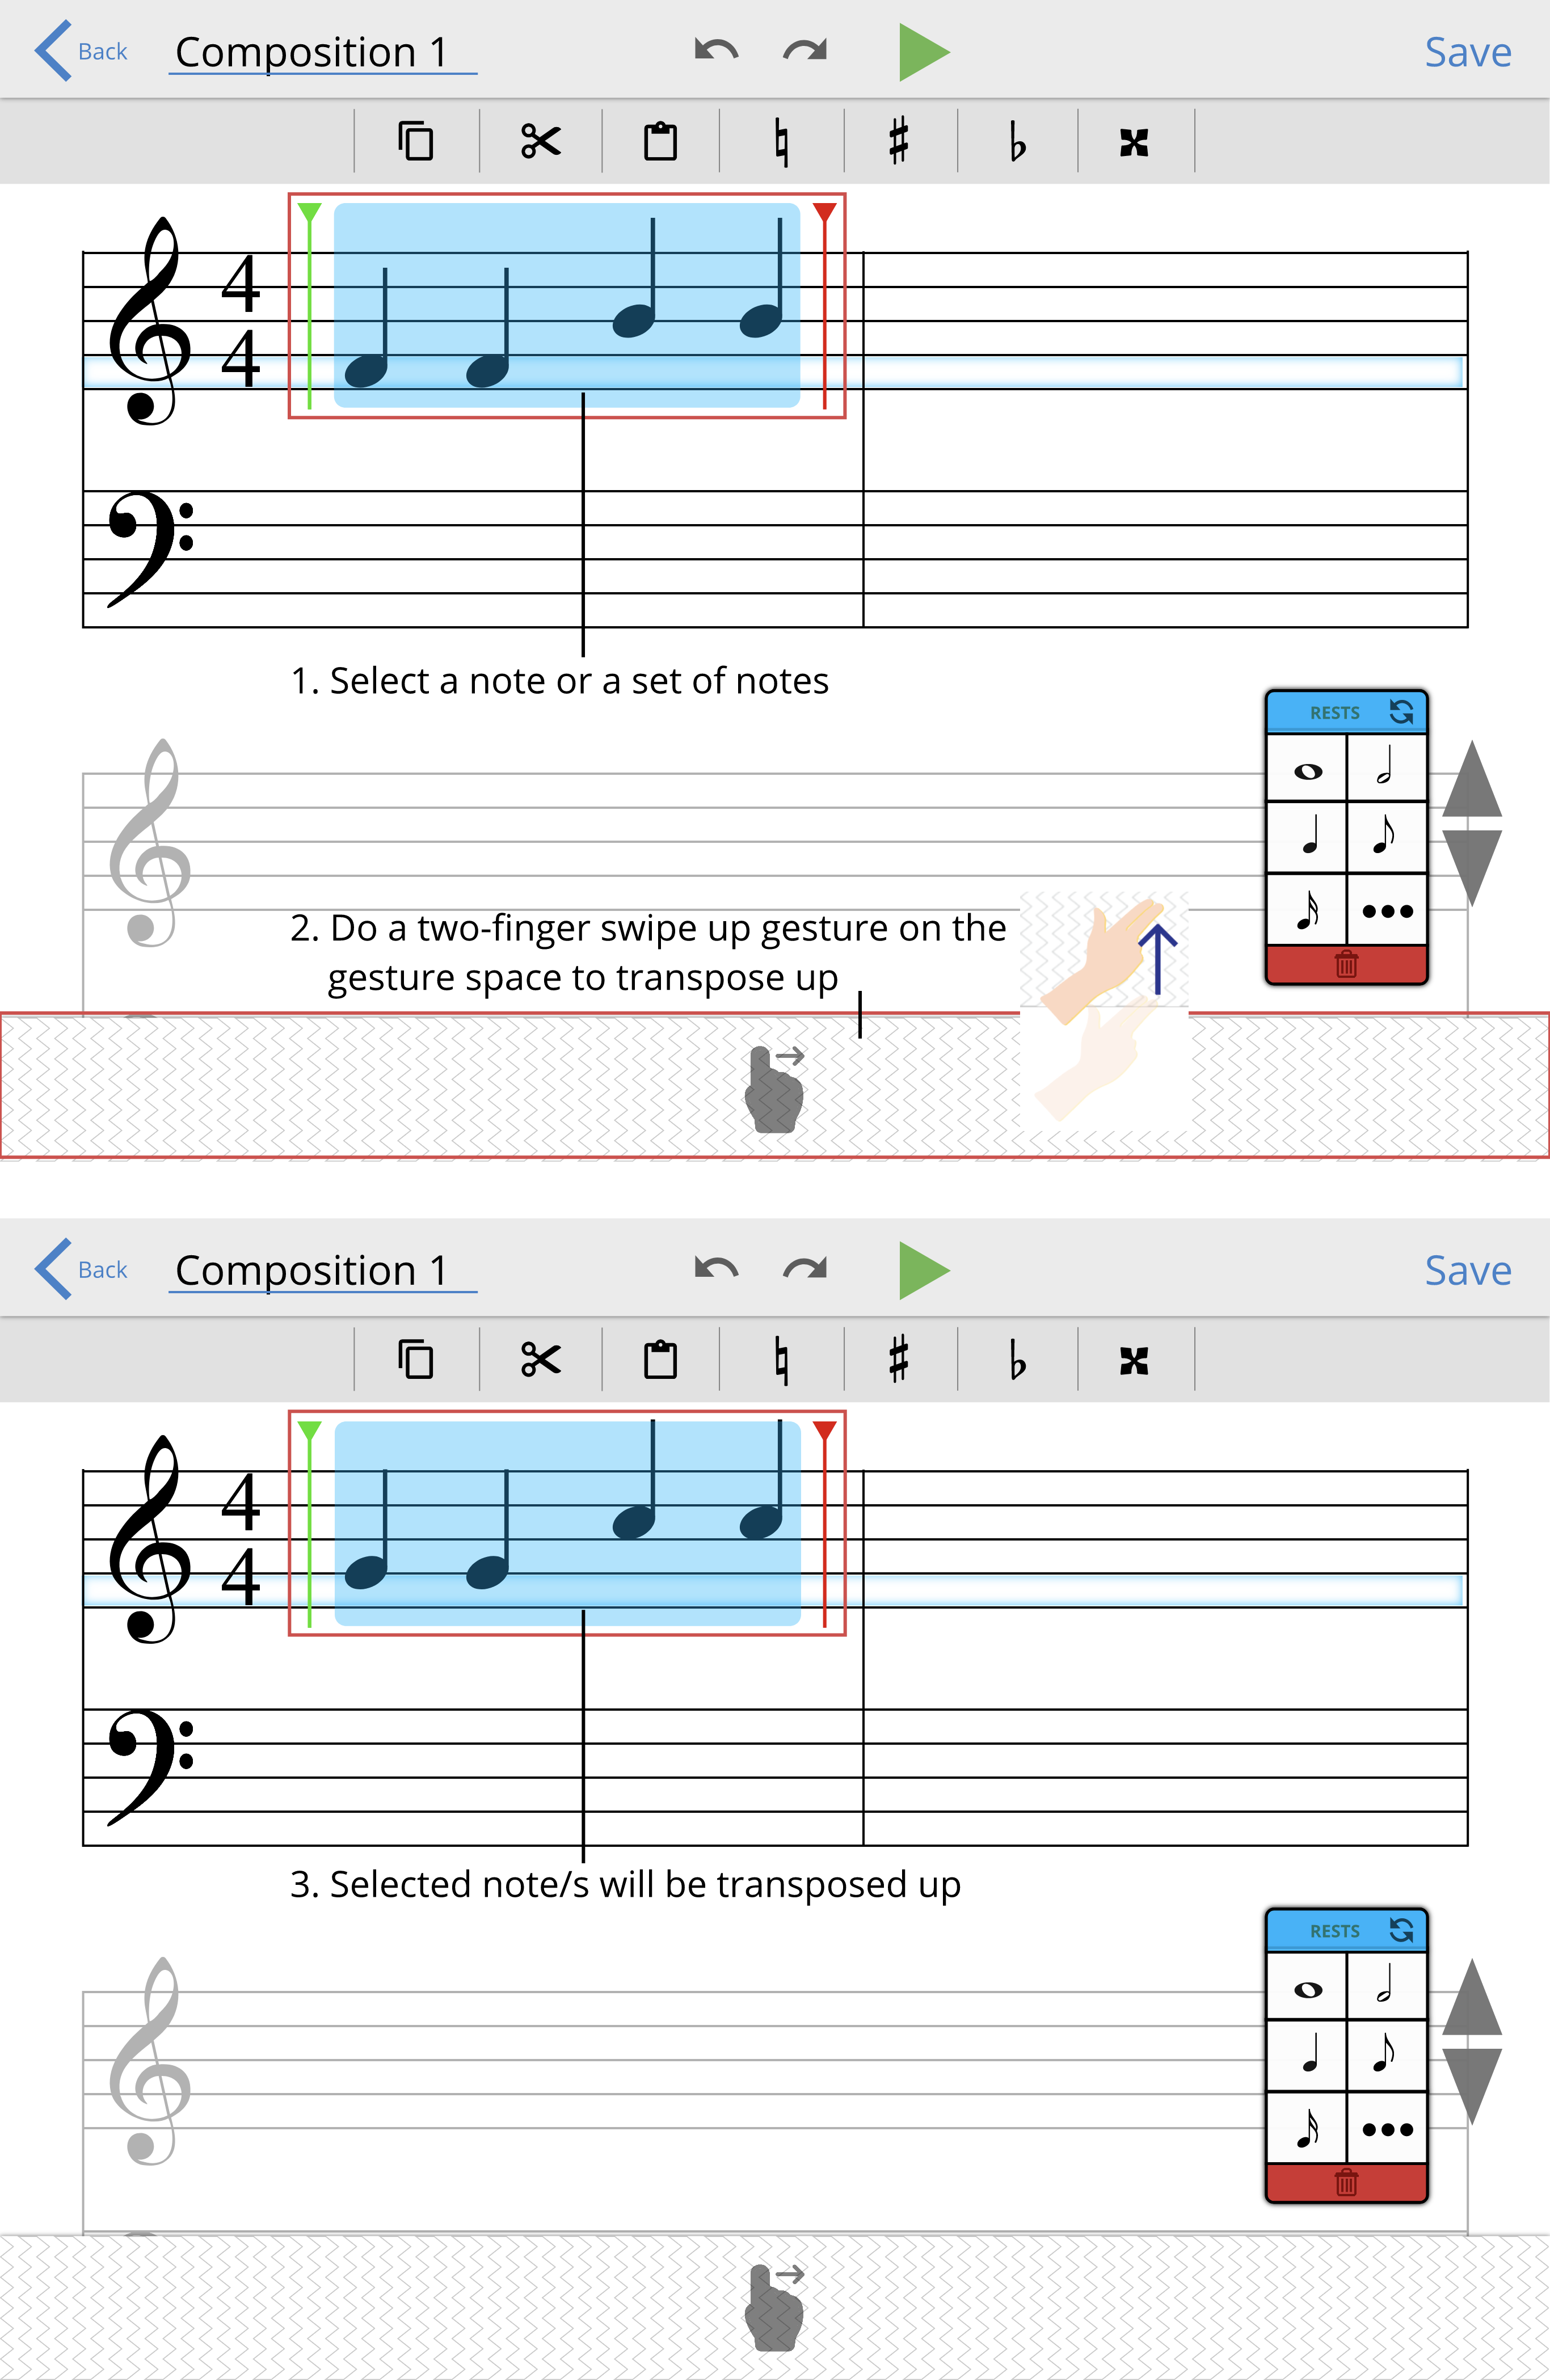
\includegraphics[scale=0.28]{Transposing_Notes}
    \label{fig:transpose-notes}
    \caption{Transpose notes by swiping with two fingers up or down on the gesture space.}
\end{figure}

\item Navigating Line/Space Selector

To navigate the line/space selector, the user may tap directly on the line/space. Alternatively, the user may use the arrow buttons beside the notes menu to traverse the selector on the staff.

\begin{figure}[H]
	\centering
	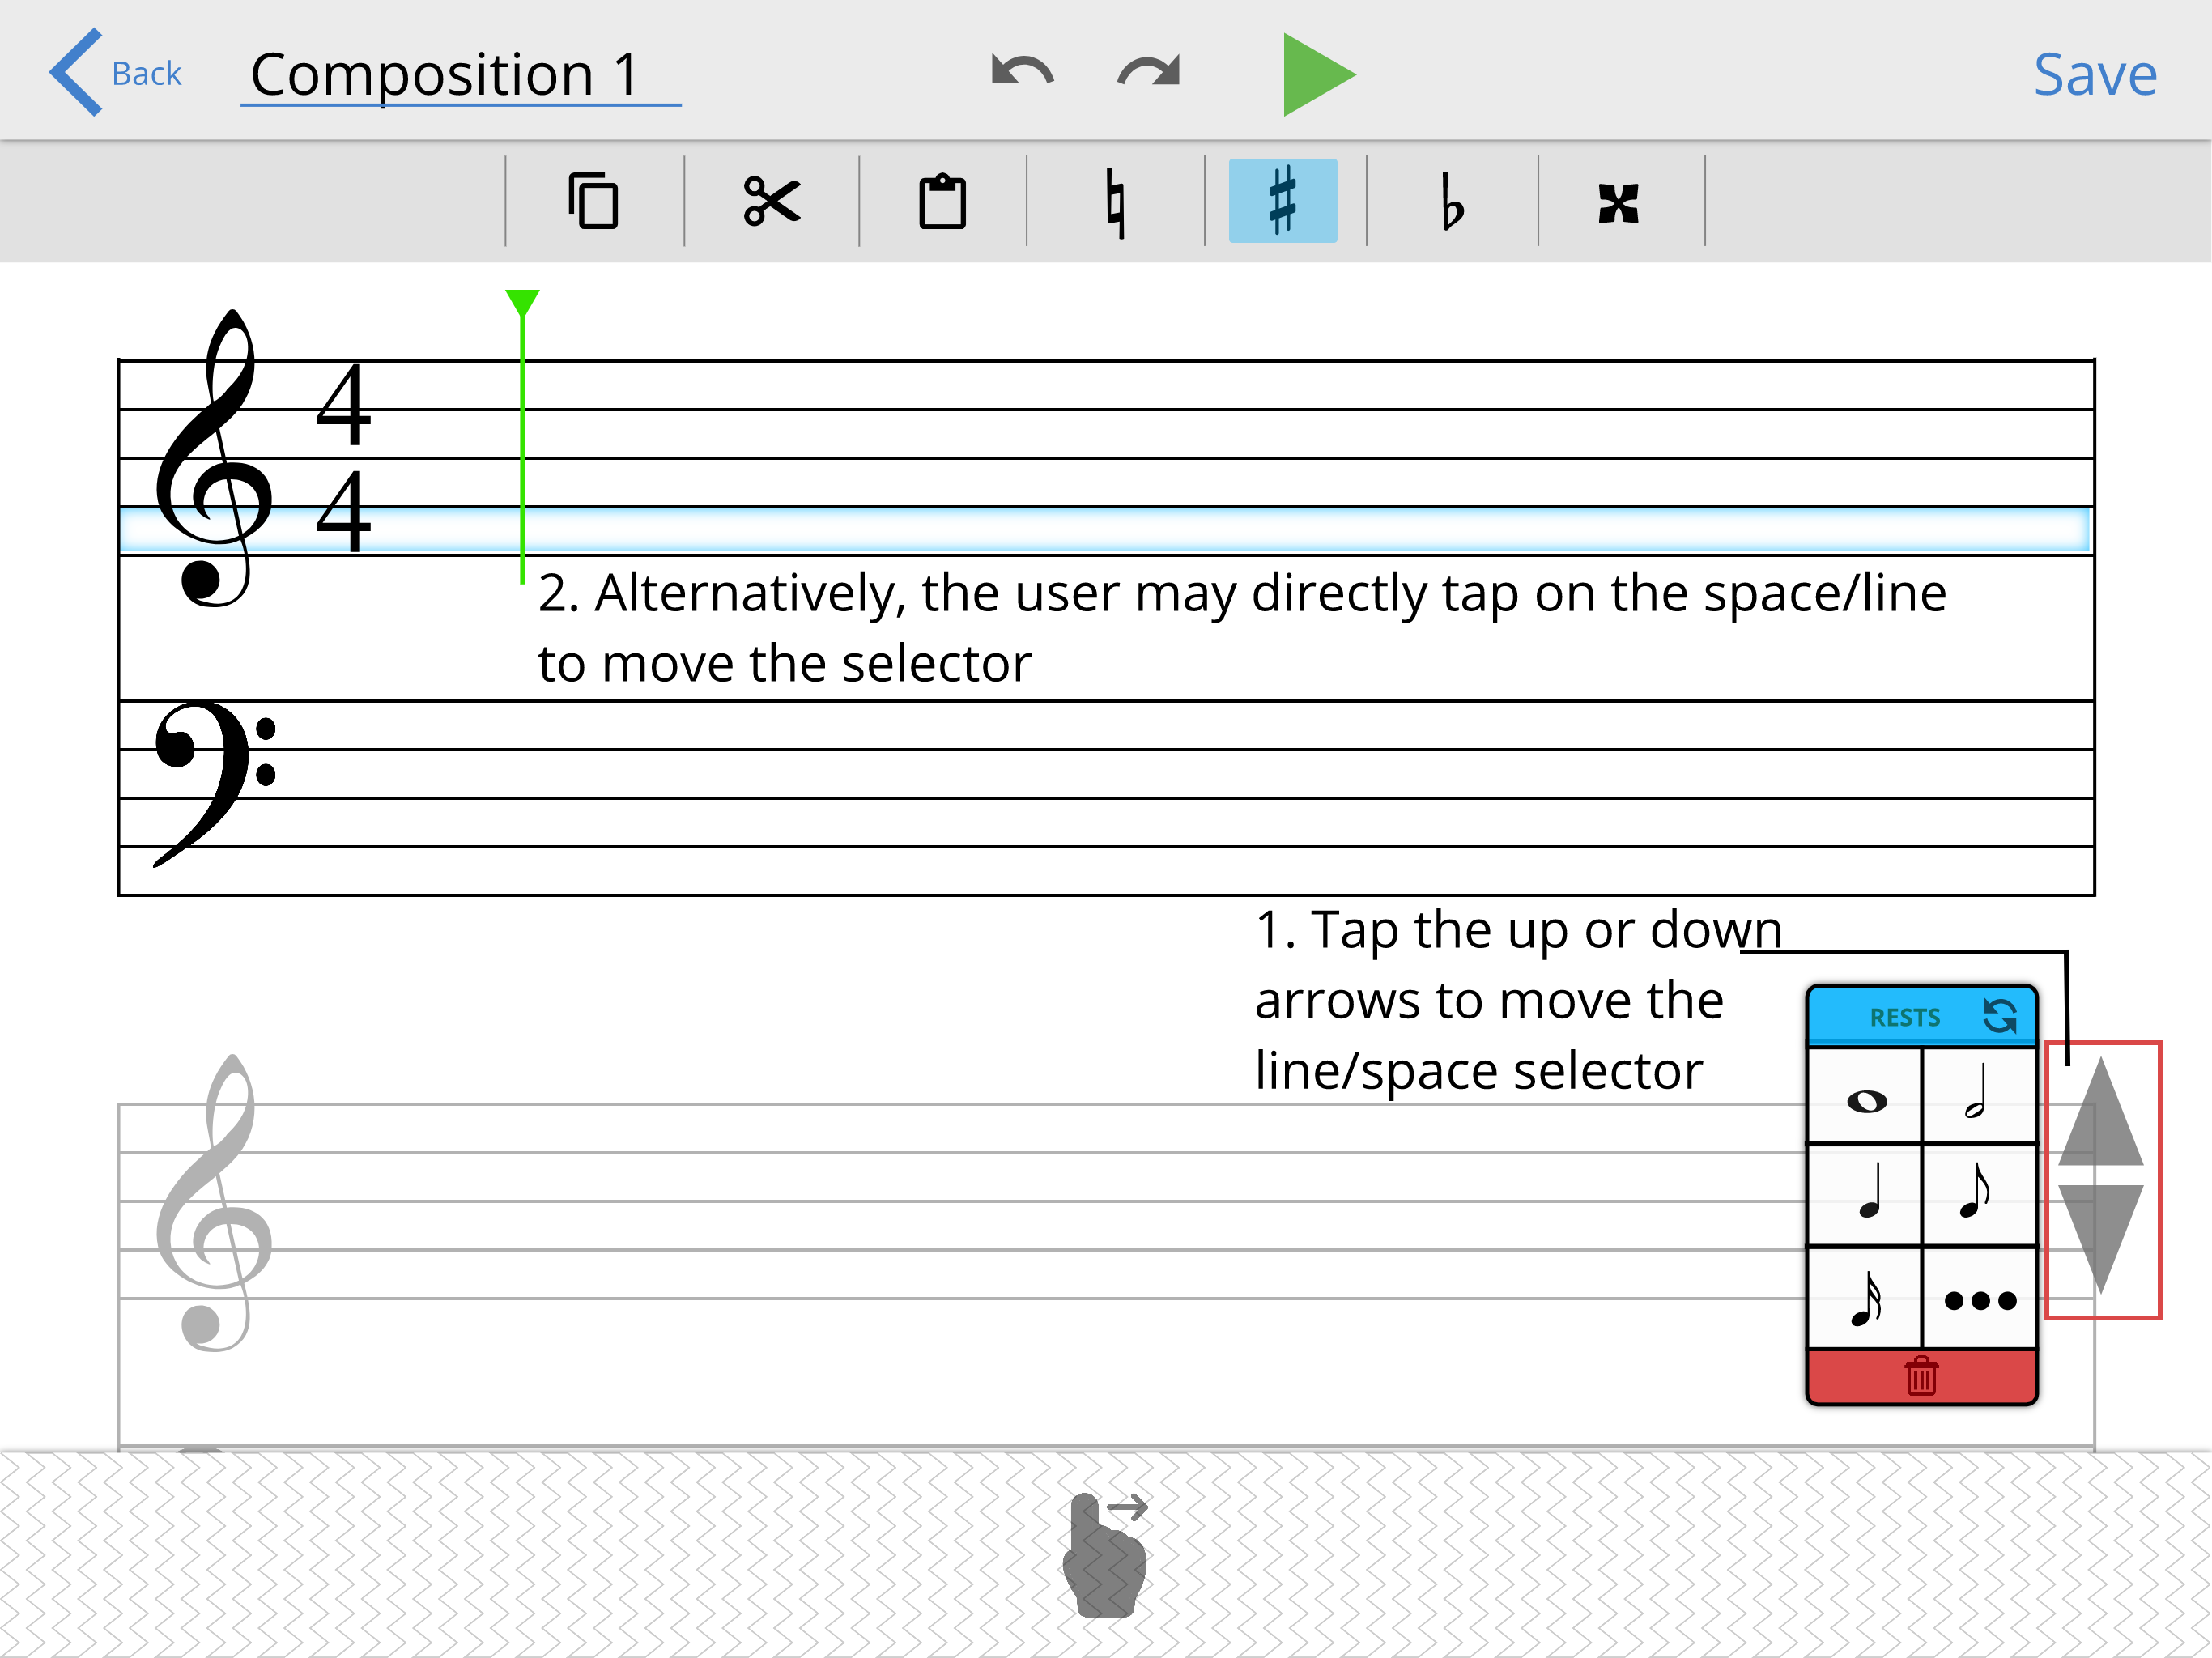
\includegraphics[scale=0.28]{Navigating}
    \label{fig:navigating}
    \caption{Tap directly on the space/line or use the arrow buttons to navigate selector.}
\end{figure}

\item Music Generation

Swipe right, up, or down on the gesture space to generate notes starting from the indicator on the staff.

\begin{figure}[H]
	\centering
	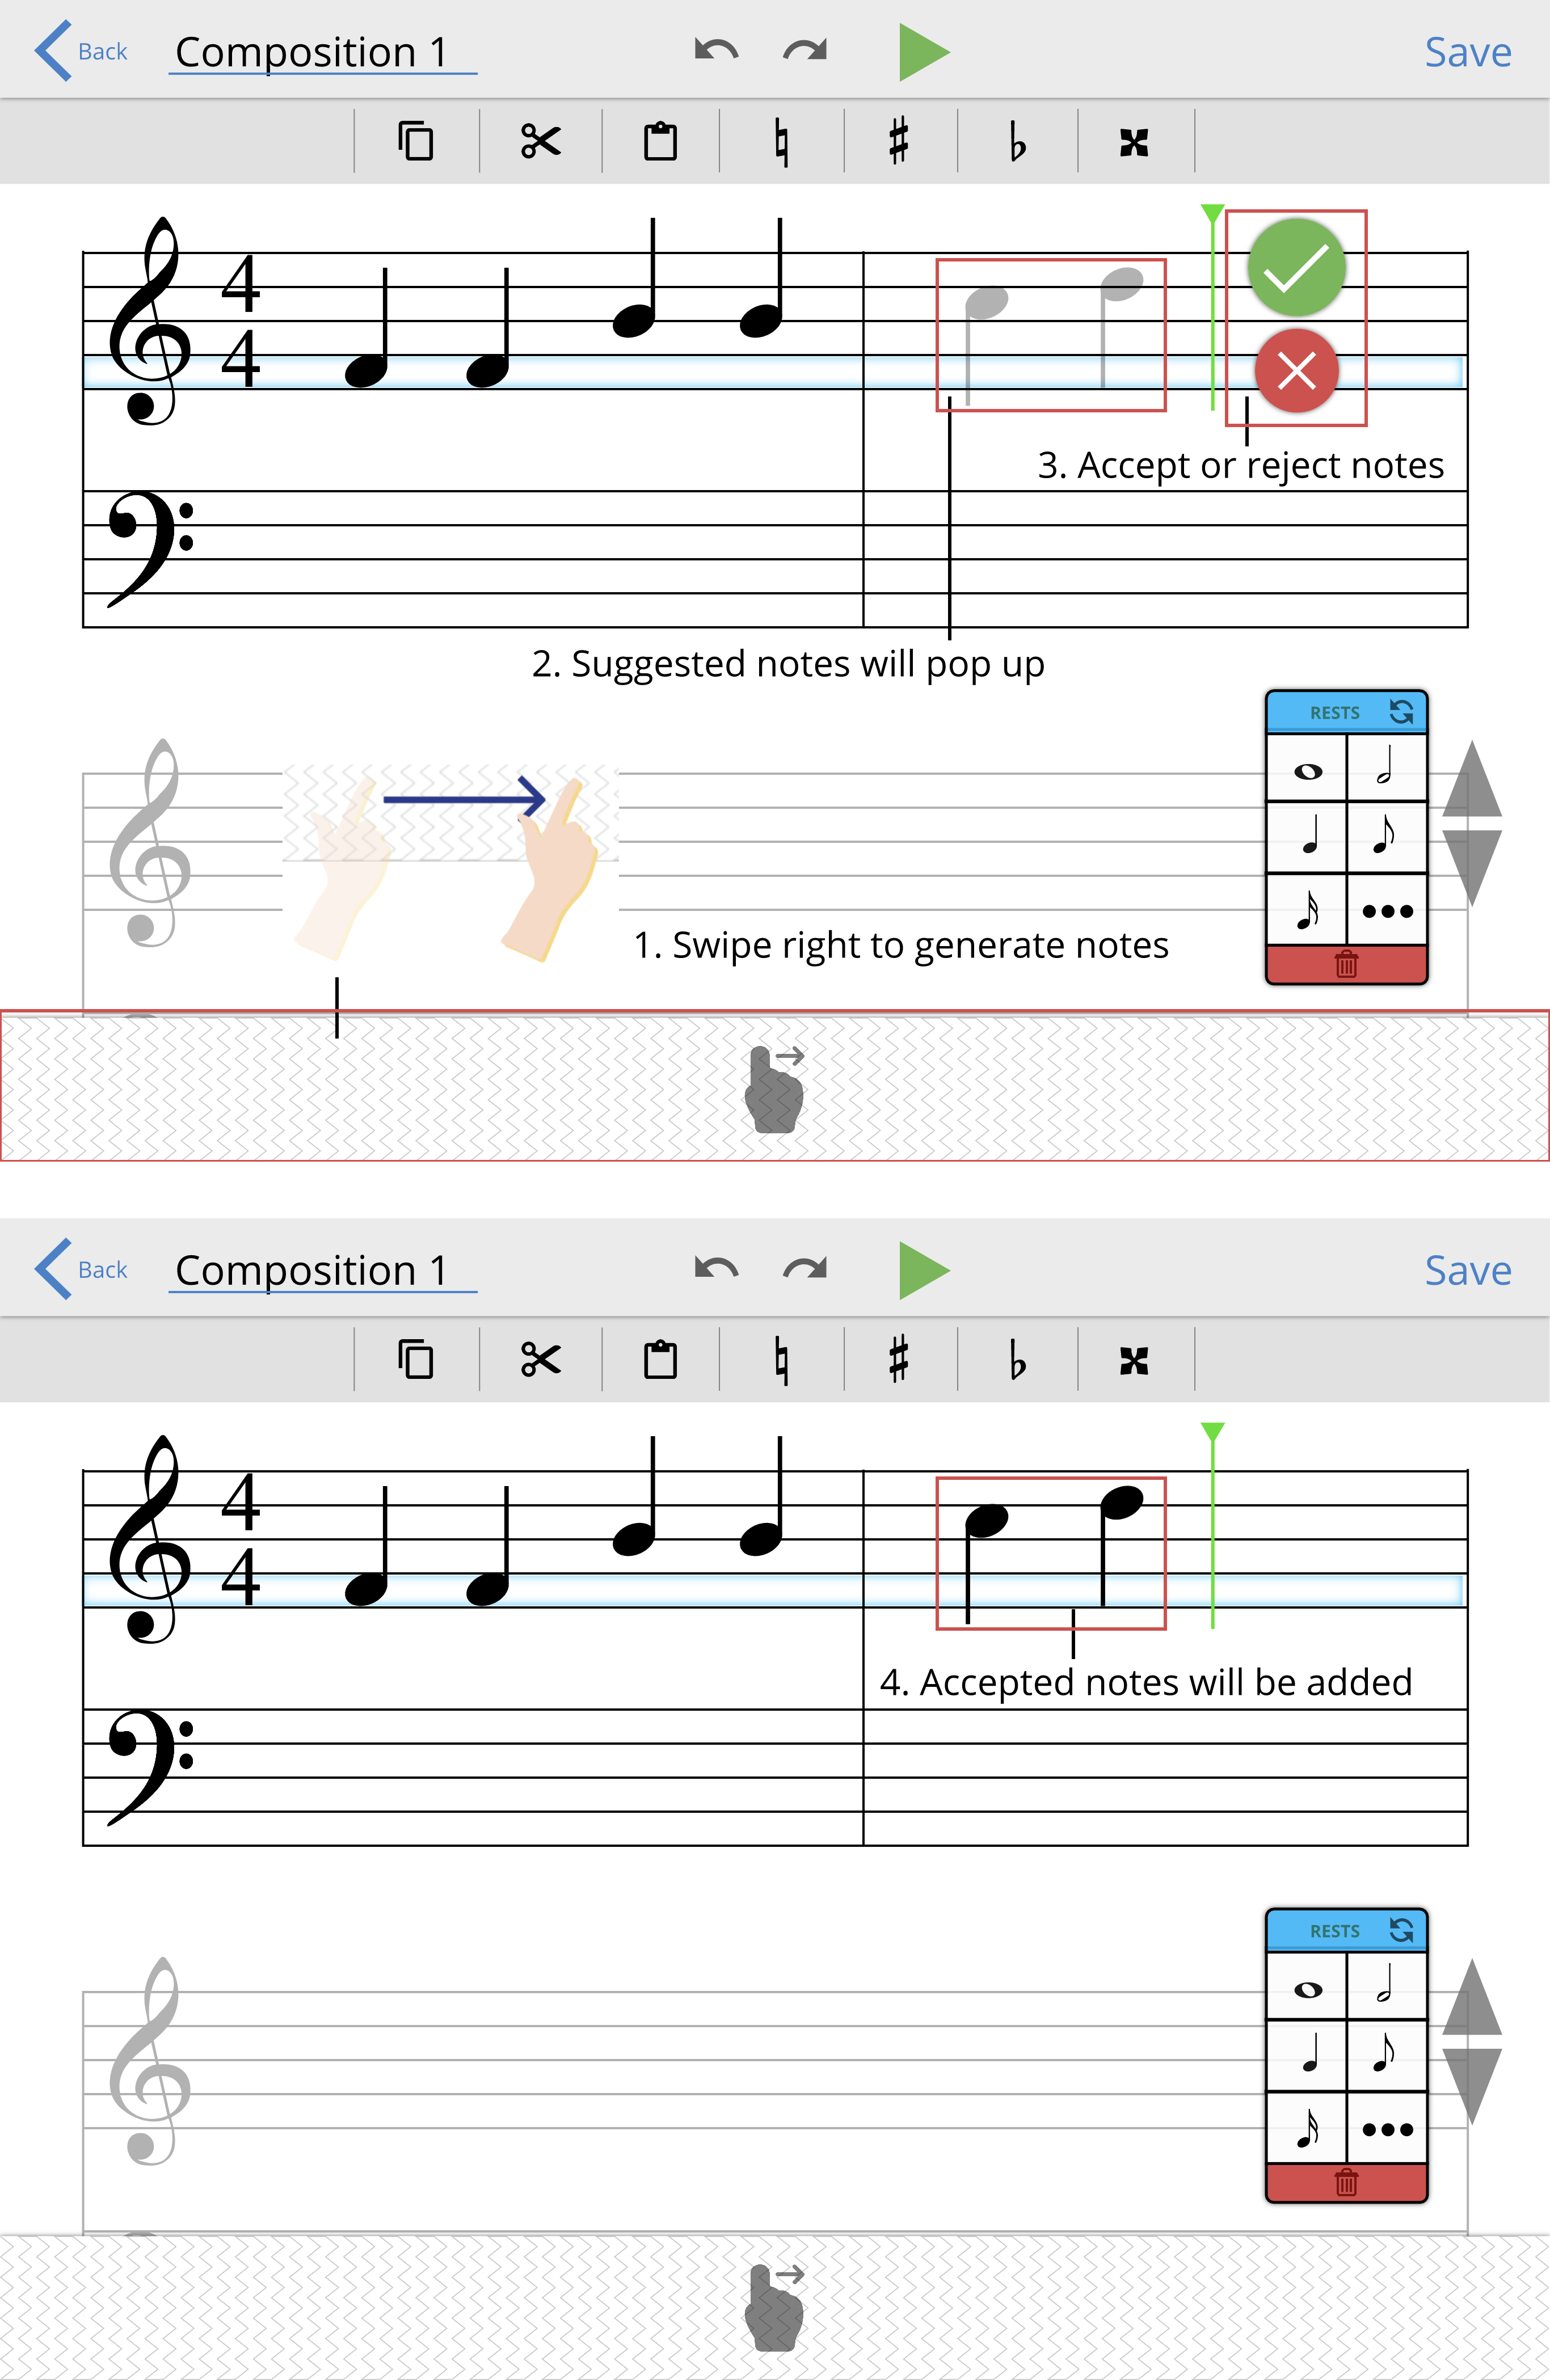
\includegraphics[scale=0.28]{Metacreation}
    \label{fig:metacreation}
    \caption{Swipe right to generate notes.}
\end{figure}

\item Note Hint - Tap a note to see the letter and octave number.

\begin{figure}[H]
	\centering
	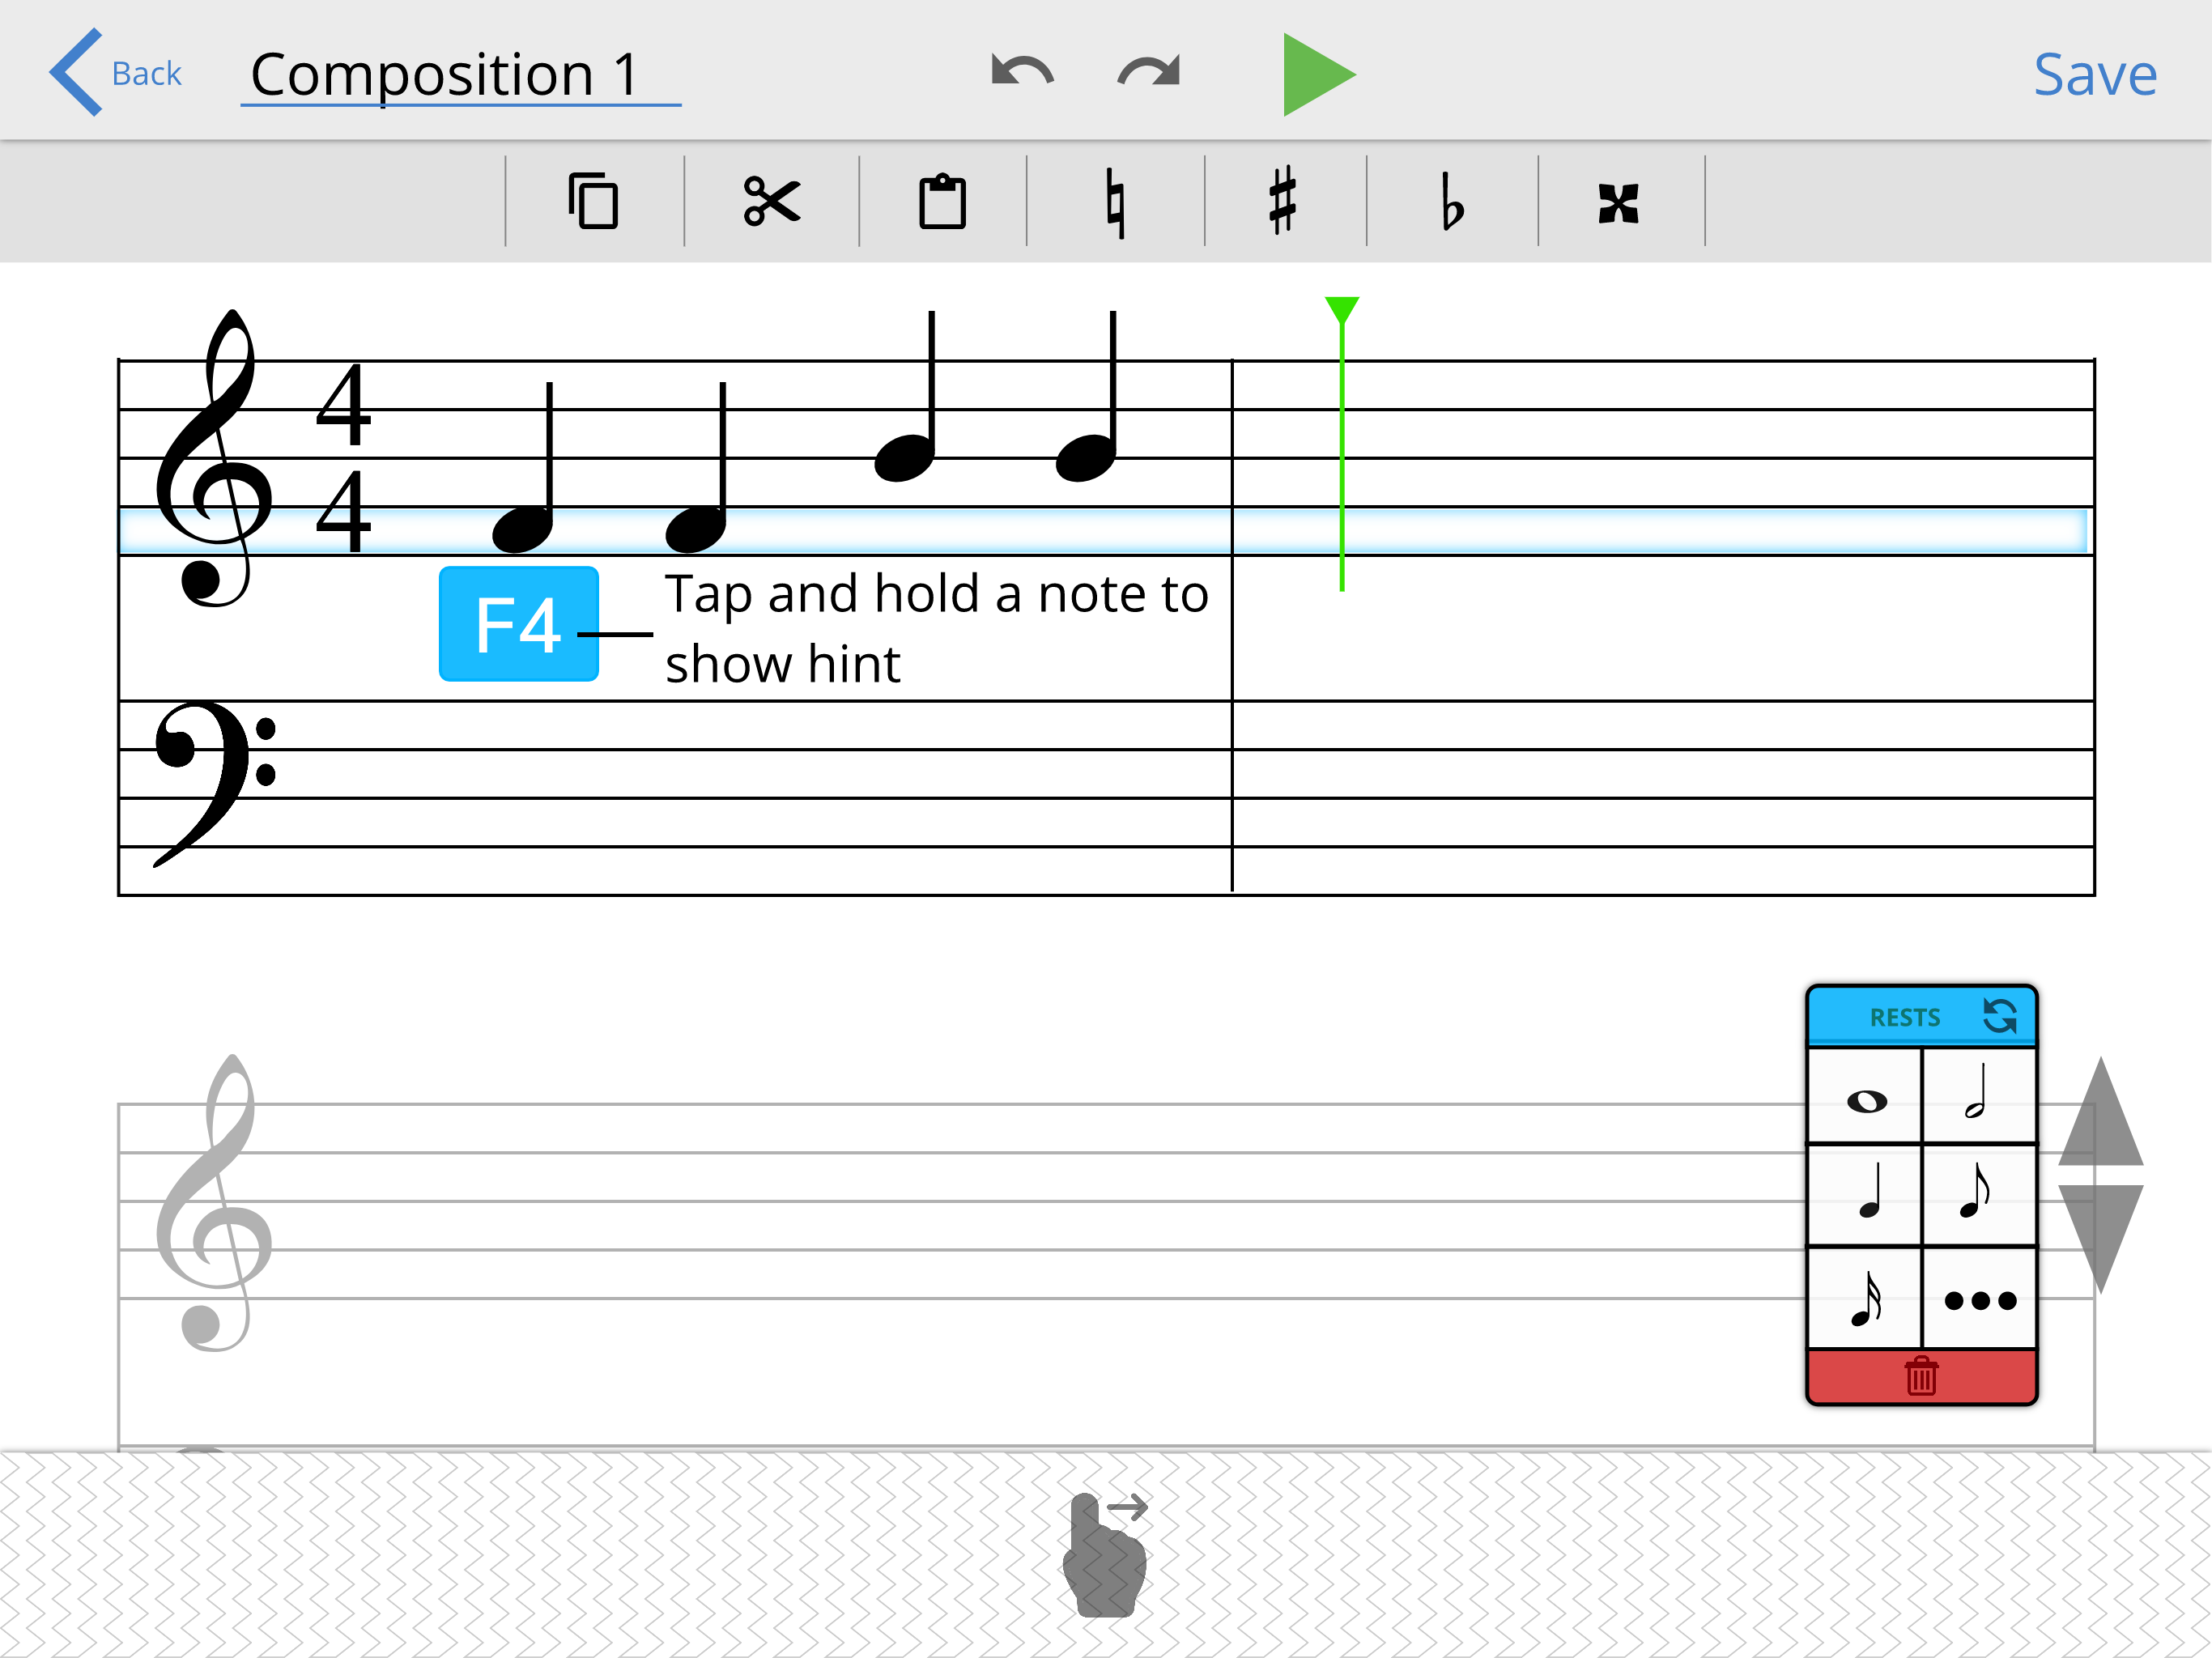
\includegraphics[scale=0.28]{Note_Hint}
    \label{fig:initialselection}
    \caption{Note details popup.}
\end{figure}

\end{enumerate}

\section{Experiment Design}

This chapter will describe the user stories and use cases that will be highlighted in the testing of the application. The intended users for the application will be expert composers who have at least 7 years of experience with composing music and amateur composers who have less than a year of experience with composing music. These users should also have a basic knowledge on musical terms. The details on the testing to be conducted on these users will also be discussed in this chapter.

\subsection{User Stories}
The user stories of the system will be focused on the main functions of the application and will highlight each specific need that the user has for the system. These user stories came from the users, representing the tasks that they need to perform on musical composition applications. These are created with the context that the system will run on a mobile platform with the mode of interaction mainly being touch gestures. 

\begin{enumerate}
\item As a user, I want to be able to create a blank composition, so that I can start my work
\item As a user, I want to be able to name my composition, so that I can differentiate it from my other compositions
\item As a user, I want to be able to save my composition, so that I can come back to it later
\item As a user, I want to be able to view all my saved compositions in a list, so that I can keep track of everything
\item As a user, I want to be able to open a saved composition so that I can perform more actions on it
\item As a user, I want to be able export my composition in a format that I can open in the composition application I use on my laptop
\item As a user, I want to be able to delete a composition, so I can discard compositions I do not work on anymore
\item As a user, I want to be able to add a chord progression in my composition, so that I do not need to individually add notes that belong to a progression
\item As a user, I want to be able to place a note in my composition, so that I can create my composition
\item As a user, I want to be able to select a single note, so that I can perform actions on it
\item As a user, I want to be able to change the pitch class of a note in my composition, so that I can make adjustments to my composition
\item As a user, I want to be able to change the type of a note in my composition, so that I can make the sound longer or shorter
\item As a user, I want to be able to erase a note in my composition, so that I can make space for other notes in my composition
\item As a user, I want to be able to highlight a group of notes in my composition, so that I can perform actions on the group
\item As a user, I want to be able to erase a highlighted group of notes in my composition, so that I can make space faster for other notes I'd like to place in my composition
\item As a user, I want to be able to place a rest in my composition, so I can have pauses in my composition
\item As a user, I want to be able to select a rest, so that I can perform actions on that rest
\item As a user, I want to be able to change the type of rest, so that I can change the length of pauses
\item As a user, I want to be able to highlight a group of rests, so that I can perform actions on the group of rests
\item As a user, I want to be able to erase a rest in my composition, so that I can make space for other rests or notes
\item As a user, I want to be able to change a rest in my composition, so that I can make adjustments to my composition
%\item As a user, I want to be able to move the position of a note in my composition, so that I can move that note to a better position
%\item As a user, I want to be able to move the position of a highlighted group of notes in my composition, so that I can reposition multiple notes at a time to a better position
\item As a user, I want to be able to hear the sound of the note I just added, so that I know I've added the correct sounding note
\item As a user, I want to be able to listen to a highlighted section of my composition, so that I can hear just a segment of my piece
\item As a user, I want to be able to listen to my whole composition, so that I can hear it as a whole
\item As a user, I want to be able to perform a swipe gesture that will generate a succession of notes based on the orientation of my gesture and my current composition because I'm interested in knowing what series of notes match my current composition
\item As a user, I want to be able to manipulate the generated series of notes, because the generated series of notes just needs a little bit more adjustments before I accept it into my composition
\item As a user, I want to be able to discard the series of notes generated by the application after a swipe gesture, so I do not have to delete them one by one
\item As a user, I want to be able to confirm the addition of the series of notes given by the application after a swipe gesture, so I can create my composition quickly
\item As a user I want to be able to undo an action or a series of actions, so that I can undo an unintended action or series of unintended actions quicker
\item As a user I want to be able to redo an action or a series of actions, so that I can redo an intended action or a series of intended actions quicker
\item As a user, I want to be able to reposition the menu because I want to place it where it is not an obstacle for me while composing
\item As a user, I want to be able to set the time signature of my composition
\item As a user, I want to be able to see the details of a single note, so that I can know the specifications of the note
\item As a user, I want to be able to see the details of a selected group of notes, so that I can know the specification of the selected group of notes
\item As a user, I want to be able to see the details of the generated series of notes like the pitch and type so that I can know what notes the system has generated after a gesture
\item As a user, I want to be able to set the clef of my composition
\item As a user, I want to be able to set the key signature of my composition
\item As a user, I want to be able to set the time signature of my composition
\item As a user, I want to be able to copy a highlighted group of notes and/or rests, so that I can copy a recurring segment in my composition
\item As a user, I want to be able to cut a highlighted group of notes and/or rests, so that I can copy a segment of my composition while at the same time making space for more notes
\item As a user, I want to be able to paste the copied or cut group of notes and/or rests onto my composition, so that I do not need to add a recurring segment in my composition manually all the time
%\item As a user, I want to be able to move the position of a rest, so that I can move that rest to a better position
%\item As a user, I want to be able to move the position of a selected group of rests, so that I can move multiple rests at a time to a better position
\item As a user, I want to be able to add accidentals to my notes, so that I can control the pitch of my notes
\item As a user, I want to be able to transpose a highlighted group of notes, so that I do not need to individually change the pitch of each note
\item As a user, I want to be able to perform retrograde inversion on a single note, so that I do not have to move it manually to invert it
\item As a user, I want to be able to perform retrograde inversion on a group of notes, so that I do not need to invert each note individually

\end{enumerate}

\subsection{Use Cases}

This section defines the several actions the users can perform within the system. These use cases were derived from the needs of the composers and the functions of Flow. The design of each use case will be based on fully dressed use cases with precision level 2 found in the book of \cite{alistair2001writing}. The headers used in each use case will be the the trigger, primary actor, supporting actors, preconditions, minimal guarantees, success guarantees, and process steps.

%Trigger
%Primary Actor
%Supporting Actors
%Precondition
%Process Steps
%Minimal Guarantees
%Success Guarantees


%%Layout needs to be fixed

%Sprint 1
\subsubsection{Use Case 1: Add a Single Note}

\begin{tabularx}{\textwidth}{|X|X|}
\hline
Trigger & The composer needs to add a note \\
\hline
Primary Actor & 
Composer \\
\hline
Supporting Actors & 
\begin{itemize}
\item Listener
\item Instrumentalist
\item Producer
\end{itemize} \\
\hline
Preconditions & 
\begin{itemize}
\item The user has a composition environment open in Flow 
\item The addition is valid based on musical rules
\end{itemize} \\
\hline
Process Steps & 
\begin{enumerate}
\item User taps on  indicator and line/space selector to a desired location along the musical staff
\item User taps on the desired note to add in the indicated location from the side menu
\end{enumerate} \\
\hline
Minimal Guarantees & 
A note will be added \\
\hline
Success Guarantees & 
The desired note is added to the indicated location \\
\hline
Quality Requirements &  
\begin{itemize}
\item Note should be in the valid position
\item The addition of the note should be valid according to the musical rules
\end{itemize} \\ 
\hline
\end{tabularx}

%Sprint 1
\subsubsection{Use Case 2: Change a Single Note}

\begin{tabularx}{\textwidth}{|X|X|}
\hline
Trigger & 
The composer needs to change a note \\
\hline
Primary Actor & 
Composer\\
\hline
Supporting Actors & 
\begin{itemize}
\item Listener
\item Instrumentalist
\item Producer
\end{itemize} \\
\hline
Precondition & 
\begin{itemize}
\item The user has  a composition environment open in Flow  
\item The change is valid based on music rules
\end{itemize} \\
\hline
Process Steps & 
\begin{enumerate}
\item User selects the note to be changed 
\item User taps the desired note from the note menu to replace the selected note
\end{enumerate} \\
\hline
Minimal Guarantees & 
A note will be changed \\
\hline
Success Guarantees & 
The selected note will be changed \\
\hline
Quality Requirements & 
\begin{itemize}
\item The change should not violate music rules
\end{itemize} \\ 
\hline
\end{tabularx}


%Sprint 1
\subsubsection{Use Case 3: Delete a Single Note}

\begin{tabularx}{\textwidth}{|X|X|}
\hline
Trigger & 
The composer needs to delete a note \\
\hline
Primary Actor & 
Composer\\
\hline
Supporting Actors & 
\begin{itemize}
\item Listener
\item Instrumentalist
\item Producer
\end{itemize} \\
\hline
Precondition & 
\begin{itemize}
\item The user has a composition environment open in Flow 
\item The deletion is valid based on music rules
\end{itemize} \\
\hline
Process Steps & 
\begin{enumerate}
\item User selects the note to be deleted 
\item User taps the delete option in the pop-up menu to confirm deletion
\end{enumerate} \\
\hline
Minimal Guarantees & 
A note will be deleted \\
\hline
Success Guarantees & 
The correct note will be deleted \\
\hline
Quality Requirements & 
\begin{itemize}
\item Deletion of note should not violate music rules
\end{itemize} \\ 
\hline
\end{tabularx}

\subsubsection{Use Case 4: Horizontal Swipe Gesture to Generate a series of Notes}

\LTXtable{\textwidth}{longtables/use_case_4_lt}

\subsubsection{Use Case 5: Add a Single Rest}

\begin{tabularx}{\textwidth}{|X|X|}
\hline
Trigger &
The composer needs to add a rest \\
\hline
Primary Actor &
Composer \\
\hline
Supporting Actors & 
\begin{itemize}
\item Listener
\item Instrumentalist
\item Producer
\end{itemize} \\
\hline
Precondition & 
\begin{itemize}
\item The user has a composition environment open in Flow
\item The addition is valid based on musical rules
\end{itemize} \\
\hline
Process Steps & 
\begin{enumerate}
\item User positions the indicator to a desired location along the musical staff
\item User taps on the toggle button on the side menu to open the selection of rests
\item User taps on the desired rest to add in the indicated location from the side menu
\end{enumerate} \\
\hline
Minimal Guarantees & 
A rest will be added \\
\hline
Success Guarantees & 
The desired rest is added to the indicated location \\
\hline
Quality Requirements & 
\begin{itemize}
\item Rest should be in the valid position
\item The addition of the rest should be valid according to the musical rules
\end{itemize} \\ 
\hline
\end{tabularx}

\subsubsection{Use Case 6: Delete a Highlighted Group of Notes or Rests}

\begin{tabularx}{\textwidth}{|X|X|}
\hline
Trigger & 
The user needs to delete a group of notes \\
\hline
Primary Actor & 
Composer \\
\hline
Supporting Actors & 
\begin{itemize}
\item Listener
\item Instrumentalist
\item Producer
\end{itemize} \\
\hline
Precondition & 
\begin{itemize}
\item The user has a composition environment open in Flow
\item The group deletion is valid based on musical rules
\end{itemize} \\
\hline
Process Steps & 
\begin{enumerate}
\item User highlights a group of notes
\item User taps the delete option in the side menu
\end{enumerate} \\
\hline
Minimal Guarantees & 
A group of notes will be deleted \\
\hline
Success Guarantees & 
The highlighted group of notes will be deleted \\
\hline
Quality Requirements & 
\begin{itemize}
\item The deletion of the group of notes does not violate the musical rules
\item The group of notes will be removed from the composition environment
\end{itemize} \\ 
\hline
\end{tabularx}

\subsubsection{Use Case 7: View the Details of a Single Note or Rest}

\begin{tabularx}{\textwidth}{|X|X|}
\hline
Trigger & 
The user wants to know the details of a particular note or rest\\
\hline
Primary Actor & 
Composer \\
\hline
Supporting Actors & 
\begin{itemize}
\item Listener
\item Instrumentalist
\item Producer
\end{itemize} \\
\hline
Precondition & 
\begin{itemize}
\item The user has a composition environment open in Flow
\item The note or rest exists within the composition
\end{itemize} \\
\hline
Process Steps & 
\begin{enumerate}
\item The user selects a note or rest
\item The user taps on the toggle details option
\end{enumerate} \\
\hline
Minimal Guarantees & 
The toggle button graphic will change\\
\hline
Success Guarantees & 
The toggle button graphic will change and details of the selected note or rest will be displayed \\
\hline
Quality Requirements & 
\begin{itemize}
\item The details displayed about the selected note or rest should be correct
\item The toggle button icon should be correct
\end{itemize} \\ 
\hline
\end{tabularx}


\subsubsection{Use Case 8: View the Details of a Highlighted Group of Notes or Rests}

\begin{tabularx}{\textwidth}{|X|X|}
\hline
Trigger & 
The user needs to view the details of a group of notes \\
\hline
Primary Actor & 
Composer \\
\hline
Supporting Actors & 
\begin{itemize}
\item Listener
\item Instrumentalist
\item Producer
\end{itemize} \\
\hline
Precondition & 
\begin{itemize}
\item The user has a composition environment open in Flow
\item The group of notes or rests exists
\end{itemize} \\
\hline
Process Steps & 
\begin{enumerate}
\item The user highlights a group of notes or rests
\item The user taps on the toggle details option 
\end{enumerate} \\
\hline
Minimal Guarantees & 
The toggle button graphic will change \\
\hline
Success Guarantees & 
The toggle button graphic will change and the details of the group of notes or rests will be displayed\\
\hline
Quality Requirements & 
\begin{itemize}
\item The information displayed about the group of notes or rests should be correct
\item The toggle button icon should be correct 
\end{itemize} \\ 
\hline
\end{tabularx}

\subsubsection{Use Case 9: Listen to the Whole Composition}

\begin{tabularx}{\textwidth}{|X|X|}
\hline
Trigger & 
The user wants to listen to the whole composition \\
\hline
Primary Actor & 
Composer \\
\hline
Supporting Actors & 
\begin{itemize}
\item Listener
\item Instrumentalist
\item Producer
\end{itemize} \\
\hline
Precondition & 
\begin{itemize}
\item The user has a composition environment open in Flow
\item The composition is not empty
\end{itemize} \\
\hline
Process Steps & 
\begin{enumerate}
\item The user taps on the play button
\end{enumerate} \\
\hline
Minimal Guarantees & 
A note will be played \\
\hline
Success Guarantees & 
The whole composition will be played correctly \\
\hline
Quality Requirements & 
\begin{itemize}
\item There should be no incorrect notes or rest played
\item The playing should only conclude after the last note or rest is played
\end{itemize} \\ 
\hline
\end{tabularx}

\subsubsection{Use Case 10: Listen to a Highlighted Section of the Composition}

\begin{tabularx}{\textwidth}{|X|X|}
\hline
Trigger & 
The user only wants to hear a section of the composition \\
\hline
Primary Actor & 
Composer \\
\hline
Supporting Actors & 
\begin{itemize}
\item Listener
\item Instrumentalist
\item Producer
\end{itemize} \\
\hline
Precondition & 
\begin{itemize}
\item The user has a composition environment open in Flow
\item The composition is not empty
\item The highlighted section contains at least one note or rest
\end{itemize} \\
\hline
Process Steps & 
\begin{enumerate}
\item The user highlights a section of the composition
\item The user taps the play button
\end{enumerate} \\
\hline
Minimal Guarantees & 
A note will be played \\
\hline
Success Guarantees & 
The highlighted section will be played correctly \\
\hline
Quality Requirements & 
\begin{itemize}
\item There should be no incorrect note or rest played
\item The playing should only conclude after the last note or rest in the highlighted section is played
\end{itemize} \\ 
\hline
\end{tabularx}

%Sprint 1
\subsubsection{Use Case 11: Create Blank Composition}

\LTXtable{\textwidth}{longtables/use_case_11_lt}

%Sprint 1
\subsubsection{Use Case 12: View Existing Composition}

\begin{tabularx}{\textwidth}{|X|X|}
\hline
Trigger & 
The composer needs to view an existing composition \\
\hline
Primary Actor & 
Composer \\
\hline
Supporting Actors & 
\begin{itemize}
\item Listener
\item Instrumentalist
\item Producer
\end{itemize} \\
\hline
Precondition & 
\begin{itemize}
\item The user is in the main menu screen
\item The composition is in storage and is not corrupted
\end{itemize} \\
\hline
Process Steps & 
\begin{enumerate}
\item User edit composition option from the main menu
\end{enumerate} \\
\hline
Minimal Guarantees & 
A composition will open \\
\hline
Success Guarantees & 
The selected composition will open \\
\hline
Quality Requirements &
\begin{itemize}
\item The opened composition should have all the previous elements placed before in the correct position
\end{itemize} \\ 
\hline
\end{tabularx}

%Sprint 1
\subsubsection{Use Case 13: Delete Existing Composition}

\begin{tabularx}{\textwidth}{|X|X|}
\hline
Trigger & 
The composer needs to delete a composition \\
\hline
Primary Actor & 
Composer \\
\hline
Supporting Actors & 
\begin{itemize}
\item Listener
\item Instrumentalist
\item Producer
\end{itemize} \\
\hline
Precondition & 
\begin{itemize}
\item The user is in the main menu screen
\item The composition is in storage and is not corrupted
\end{itemize} \\
\hline
Process Steps & 
\begin{enumerate}
\item User taps delete composition option from the main menu
\item User taps confirm
\end{enumerate} \\
\hline
Minimal Guarantees & 
A composition will be deleted \\
\hline
Success Guarantees & 
The correct composition will be deleted and will not remain in the system memory \\
\hline
Quality Requirements &
\begin{itemize}
\item Composition should absolutely be gone from the system memory
\item Composition name will be made available for future compositions
\end{itemize} \\ 
\hline
\end{tabularx}

\subsubsection{Use Case 14: Redo an Action}

\begin{tabularx}{\textwidth}{|X|X|}
\hline
Trigger & 
The user wants to redo an action\\
\hline
Primary Actor & 
Composer \\
\hline
Supporting Actors & 
\begin{itemize}
\item Listener
\item Instrumentalist
\item Producer
\end{itemize} \\
\hline
Precondition & 
\begin{itemize}
\item An undo action has been performed at least once
\item Action can be redone
\end{itemize} \\
\hline
Process Steps & 
\begin{enumerate}
\item The user taps on the redo button
\end{enumerate} \\
\hline
Minimal Guarantees & 
The redo button will give feedback \\
\hline
Success Guarantees & 
The action is redone\\
\hline
Quality Requirements & 
\begin{itemize}
\item The redone action is the correct one 
\end{itemize} \\ 
\hline
\end{tabularx}

\subsubsection{Use Case 15: Undo an Action}

\begin{tabularx}{\textwidth}{|X|X|}
\hline
Trigger & 
The user wants to undo an action \\
\hline
Primary Actor & 
Composer \\
\hline
Supporting Actors & 
\begin{itemize}
\item Listener
\item Instrumentalist
\item Producer
\end{itemize} \\
\hline
Precondition & 
\begin{itemize}
\item At least one action has been performed
\item Action can be undone
\end{itemize} \\
\hline
Process Steps & 
\begin{enumerate}
\item The user taps on the undo button
\end{enumerate} \\
\hline
Minimal Guarantees & 
The undo button will give feedback \\
\hline
Success Guarantees & 
The action is undone \\
\hline
Quality Requirements & 
\begin{itemize}
\item The undone action is the correct one 
\end{itemize} \\ 
\hline
\end{tabularx}


\subsubsection{Use Case 16: Highlight a Group of Notes or Rests}

\begin{tabularx}{\textwidth}{|X|X|}
\hline
Trigger & 
The user wants to highlight a group of notes or rests \\
\hline
Primary Actor & 
Composer \\
\hline
Supporting Actors & 
\begin{itemize}
\item Listener
\item Instrumentalist
\item Producer
\end{itemize} \\
\hline
Precondition & 
\begin{itemize}
\item The user has a composition environment open in Flow
\item The section to be highlighted contains at least one note or rest
\end{itemize} \\
\hline
Process Steps & 
\begin{enumerate}
\item The user highlights a section of the composition
\end{enumerate} \\
\hline
Minimal Guarantees & 
None \\
\hline
Success Guarantees & 
A section of the composition will be highlighted based on the gesture of the user \\
\hline
Quality Requirements & 
\begin{itemize}
\item The highlighted section should be the one the user wanted to highlight
\end{itemize} \\ 
\hline
\end{tabularx}

\subsubsection{Use Case 17: Change the Time Signature of the Composition}

\begin{tabularx}{\textwidth}{|X|X|}
\hline
Trigger & 
The user wants to change the time signature of the composition \\
\hline
Primary Actor & 
Composer \\
\hline
Supporting Actors & 
\begin{itemize}
\item Listener
\item Instrumentalist
\item Producer
\end{itemize} \\
\hline
Precondition & 
\begin{itemize}
\item The user has a composition environment open in Flow
\item The input for the new time signature follows the musical rules
\end{itemize} \\
\hline
Process Steps & 
\begin{enumerate}
\item The user taps on the time signature
\item The user inputs the desired new time signature
\item The user taps confirm
\end{enumerate} \\
\hline
Minimal Guarantees & 
The pop-up for the input of the new time signature closes \\
\hline
Success Guarantees & 
The new time signature is applied to the composition \\
\hline
Quality Requirements & 
\begin{itemize}
\item The notes and rests within the composition will adjust based on the new time signature
\end{itemize} \\ 
\hline
\end{tabularx}

\subsubsection{Use Case 18: Change a Clef}

\begin{tabularx}{\textwidth}{|X|X|}
\hline
Trigger & 
The user wants to change a clef in the composition \\
\hline
Primary Actor & 
Composer \\
\hline
Supporting Actors & 
\begin{itemize}
\item Listener
\item Instrumentalist
\item Producer
\end{itemize} \\
\hline
Precondition & 
\begin{itemize}
\item The user has a composition environment open in Flow
\item The change does not violate the musical rules
\end{itemize} \\
\hline
Process Steps & 
\begin{enumerate}
\item The user taps on a clef to change
\item The user selects the new desired clef
\item The user taps confirm
\end{enumerate} \\
\hline
Minimal Guarantees & 
The menu containing the selection of clef does not remain in the screen \\
\hline
Success Guarantees & 
The selected clef is changed into the desired clef \\
\hline
Quality Requirements & 
\begin{itemize}
\item The desired clef is in the right staff within the composition
\item The desired clef is the correct one that the user selected
\end{itemize} \\ 
\hline
\end{tabularx}

\subsubsection{Use Case 19: Change the Key Signature of the Composition}

\begin{tabularx}{\textwidth}{|X|X|}
\hline
Trigger & 
The user wants to change the key signature of the composition \\
\hline
Primary Actor & 
Composer \\
\hline
Supporting Actors & 
\begin{itemize}
\item Listener
\item Instrumentalist
\item Producer
\end{itemize} \\
\hline
Precondition & 
\begin{itemize}
\item The user has a composition environment open in Flow
\item The input for the new key signature follows the musical rules
\end{itemize} \\
\hline
Process Steps & 
\begin{enumerate}
\item The user taps on the key signature
\item The user inputs the desired new key signature
\item The user taps confirm
\end{enumerate} \\
\hline
Minimal Guarantees & 
The pop-up for the input of the new key signature closes \\
\hline
Success Guarantees & 
The new key signature is applied to the composition \\
\hline
Quality Requirements & 
\begin{itemize}
\item The notes and rests within the composition will adjust based on the new key signature
\end{itemize} \\ 
\hline
\end{tabularx}

\subsubsection{Use Case 20: Rename the Composition from the Composition Environment}

\begin{tabularx}{\textwidth}{|X|X|}
\hline
Trigger & 
The user wants to change the name of the composition \\
\hline
Primary Actor & 
Composer \\
\hline
Supporting Actors & 
\begin{itemize}
\item Listener
\item Instrumentalist
\item Producer
\end{itemize} \\
\hline
Precondition & 
\begin{itemize}
\item The user has a composition environment open in Flow
\item The new name does not violate any restrictions or limits set within Flow
\end{itemize} \\
\hline
Process Steps & 
\begin{enumerate}
\item The user taps on the name of the composition
\item The user inputs the new name of the composition
\item The user taps confirm
\end{enumerate} \\
\hline
Minimal Guarantees & 
The pop-up for the input of the new name closes \\
\hline
Success Guarantees & 
The new name is set on the composition \\
\hline
Quality Requirements & 
\begin{itemize}
\item The name should remain the same even after Flow reboots or the composition is closed
\end{itemize} \\ 
\hline
\end{tabularx}

\subsubsection{Use Case 21: Rename the Composition from the Main Menu}

\begin{tabularx}{\textwidth}{|X|X|}
\hline
Trigger & 
The user wants to change the name of the composition \\
\hline
Primary Actor & 
Composer \\
\hline
Supporting Actors & 
\begin{itemize}
\item Listener
\item Instrumentalist
\item Producer
\end{itemize} \\
\hline
Precondition & 
\begin{itemize}
\item The user is on the main menu screen
\item The new name does not violate any restrictions or limits set within Flow
\end{itemize} \\
\hline
Process Steps & 
\begin{enumerate}
\item The user taps on edit name option
\item The user inputs the new name of the composition
\item The user taps confirm
\end{enumerate} \\
\hline
Minimal Guarantees & 
The text box containing the name reverts back to normal and should no longer ask for user input \\
\hline
Success Guarantees & 
The new name is set on the composition \\
\hline
Quality Requirements & 
\begin{itemize}
\item The name should remain the same even after Flow reboots or the composition is closed
\end{itemize} \\ 
\hline
\end{tabularx}

\subsubsection{Use Case 22: Move the Note Menu to a Different Position}

\begin{tabularx}{\textwidth}{|X|X|}
\hline
Trigger & 
The user wants to move the note menu to a different position\\
\hline
Primary Actor & 
Composer \\
\hline
Supporting Actors & 
\begin{itemize}
\item Listener
\item Instrumentalist
\item Producer
\end{itemize} \\
\hline
Precondition & 
\begin{itemize}
\item The user has a composition environment open in Flow
\item The new location for the note menu is valid
\end{itemize} \\
\hline
Process Steps & 
\begin{enumerate}
\item The user drags the note menu to the desired location
\end{enumerate} \\
\hline
Minimal Guarantees & 
None \\
\hline
Success Guarantees & 
The note menu will move to its desired location\\
\hline
Quality Requirements & 
\begin{itemize}
\item The note menu will remain on its desired location after the user lifts his/her finger off the screen
\item The note menu will remain on its desired location even after the composition wherein the note menu was moved in is reopened
\end{itemize} \\ 
\hline
\end{tabularx}

\subsubsection{Use Case 23: Toggle Accidental while Adding Notes}

\begin{tabularx}{\textwidth}{|X|X|}
\hline
Trigger & 
The user wants to add an accidental to the next note \\
\hline
Primary Actor & 
Composer \\
\hline
Supporting Actors & 
\begin{itemize}
\item Listener
\item Instrumentalist
\item Producer
\end{itemize} \\
\hline
Precondition & 
\begin{itemize}
\item The user has a composition environment open in Flow
\item The addition of a new note with an accidental follows the musical rules
\end{itemize} \\
\hline
Process Steps & 
\begin{enumerate}
\item The user toggles accidental from the top menu
\item The user taps on a note from the side menu
\end{enumerate} \\
\hline
Minimal Guarantees & 
The graphic for the toggled accidental will change \\
\hline
Success Guarantees & 
The note with the toggled accidental will be added \\
\hline
Quality Requirements & 
\begin{itemize}
\item The note will be added with the toggled accidentals
\item The note with the accidentals will be placed on the desired location along the musical staff
\end{itemize} \\ 
\hline
\end{tabularx}

\subsubsection{Use Case 24: Export to MusicXML from the Main Menu}

\LTXtable{\textwidth}{longtables/use_case_24_lt}

\subsubsection{Use Case 25: Transpose a Single Note}

\begin{tabularx}{\textwidth}{|X|X|}
\hline
Trigger & 
The user wants to transpose a note to change its pitch \\
\hline
Primary Actor & 
Composer \\
\hline
Supporting Actors & 
\begin{itemize}
\item Listener
\item Instrumentalist
\item Producer
\end{itemize} \\
\hline
Precondition & 
\begin{itemize}
\item The user has a composition environment open in Flow
\item The transposition is valid
\end{itemize} \\
\hline
Process Steps & 
\begin{enumerate}
\item The user selects a note
\item The user gestures to transpose the note
\end{enumerate} \\
\hline
Minimal Guarantees & 
None \\
\hline
Success Guarantees & 
A note will be transposed \\
\hline
Quality Requirements & 
\begin{itemize}
\item The note is correctly transposed based on the gesture of the user
\end{itemize} \\ 
\hline
\end{tabularx}

\subsubsection{Use Case 26: Transpose a Selected Group of Notes}

\begin{tabularx}{\textwidth}{|X|X|}
\hline
Trigger & 
The user wants to transpose a selected group of note to change their pitch \\
\hline
Primary Actor & 
Composer \\
\hline
Supporting Actors & 
\begin{itemize}
\item Listener
\item Instrumentalist
\item Producer
\end{itemize} \\
\hline
Precondition & 
\begin{itemize}
\item The user has a composition environment open in Flow
\item The transposition is valid
\end{itemize} \\
\hline
Process Steps & 
\begin{enumerate}
\item The user selects group of notes
\item The user gestures to transpose the group of note
\end{enumerate} \\
\hline
Minimal Guarantees & 
None \\
\hline
Success Guarantees & 
A group of notes will be transposed \\
\hline
Quality Requirements & 
\begin{itemize}
\item The group of notes are correctly transposed based on the gesture of the user
\end{itemize} \\ 
\hline
\end{tabularx}

\subsubsection{Use Case 27: Change a Note to its Dotted Version}

\begin{tabularx}{\textwidth}{|X|X|}
\hline
Trigger & 
The user wants to change a note to its dotted version \\
\hline
Primary Actor & 
Composer \\
\hline
Supporting Actors & 
\begin{itemize}
\item Listener
\item Instrumentalist
\item Producer
\end{itemize} \\
\hline
Precondition & 
\begin{itemize}
\item The user has a composition environment open in Flow
\item The change into dotted version does not violate the musical rules
\end{itemize} \\
\hline
Process Steps & 
\begin{enumerate}
\item The user tap and holds on a selected note
\item The user hovers his/her finger on the selected dotted version
\item The user lifts his/her finger from the device screen
\end{enumerate} \\
\hline
Minimal Guarantees & 
The pop-up menu for dotted versions of the notes will close\\
\hline
Success Guarantees & 
The note will change to its selected dotted version \\
\hline
Quality Requirements & 
\begin{itemize}
\item The dotted version of the note is in the correct position along the musical staff
\item The dotted version of the note will remain even after the composition is reopened or Flow is relaunched
\end{itemize} \\ 
\hline
\end{tabularx}

\subsubsection{Use Case 28: Toggle from Note Menu to Rest Menu}

\begin{tabularx}{\textwidth}{|X|X|}
\hline
Trigger & 
The user wants to view the rest menu \\
\hline
Primary Actor & 
Composer \\
\hline
Supporting Actors & 
\begin{itemize}
\item Listener
\item Instrumentalist
\item Producer
\end{itemize} \\
\hline
Precondition & 
\begin{itemize}
\item The user has a composition environment open in Flow
\end{itemize} \\
\hline
Process Steps & 
\begin{enumerate}
\item The user taps toggle to rest menu button in the side menu
\end{enumerate} \\
\hline
Minimal Guarantees &
The toggle to rest menu button will give feedback\\
\hline
Success Guarantees & 
The rest menu will be displayed \\
\hline
Quality Requirements & 
\begin{itemize}
\item The proper rests are shown in the rest menu
\item The note menu will be replaced by the rest menu
\item The toggle note menu button will be in place of the toggle rest menu button
\end{itemize} \\ 
\hline
\end{tabularx}

\subsection{User Test Plan}

The objective of the tests will be to determine if the interaction and design of the system does not hinder the productivity of the target user. The functionality of the system will also be tested to see if there are problems that will occur while performing tasks.

The tests will be conducted in an environment where a tester would not be influenced by the researchers to ensure that their interaction with the application is as close as to a natural setting as possible. The prototypes for testing will be a mid-fidelity prototype created through the use of the InVision application, a prototyping tool, and the actual high-fidelity system developed using Swift. These prototypes will be in a table device. 

Before starting the test, testers will be given a consent form. If they agree with the terms and continue with the testing, the tasks indicated in Section \ref{sec:tasks} will be done for each test setup (indicated in Section \ref{sec:test-setups}) that is appropriate. Before the test setup where the tester uses the proposed system, they will be given a brief description along with the objectives of the system. 

The researchers will be collecting 3 kinds of data: time, cognitive load, and quality. There will be tasks that the testers will be asked to accomplish, and during and after those tasks, data will be collected. The time it takes to finish each task will be recorded. The cognitive load will be measured by using CogTool to receive a predicted cognitive load, and identifying moments of confusion for the users. After the testing, testers are then asked to answer a questionnaire to evaluate the quality of the application.

\subsubsection{Tasks}
\label{sec:tasks}

Some tasks may be omitted in different test setups when a crucial function to carry out the task is unavailable. During the final task, testers are encouraged to speak aloud their concerns and opinions regarding the application.

\begin{enumerate}
\item Add a note in the composition
\item Add a series of notes
\item Change a note
\item Compose a musical piece within 10 minutes
%\item Compose a musical piece worth 2 staffs without using gestures
\item Free roam the application for 3-5 minutes
\end{enumerate}

\subsubsection{Test Setups}
\label{sec:test-setups}

The test setups are meant to compare existing methods of composition with composition using Flow. The tasks enumerated in Section \ref{sec:tasks} will be used in each test setup whenever possible since some tasks can only be accomplished within a specific setup. 

There will be 3 different test setups to be used during user testing namely:

\begin{enumerate}
\item Tester composing using music sheets
\item Tester composing using Flow
\item Tester composing using komp
\end{enumerate}

The first setup simulates the traditional way of musical composition. This is through music sheets and a writing instrument. Traditional music sheets will be provided by the researchers as well as a choice of using a pen or pencil for writing musical elements. The composers are free to use as much music sheets as they want for drafting and experimenting with their composition as long as the time and resources provided by the researchers allow them.

The second setup will be focused on the composer using the developed system, Flow. During the early periods of testing, a mid-fidelity InVision prototype will be used as a substitute. Using this prototype, the only task that the composer will be able to do is to explore the application. The main goal of this is to develop and improve the interaction design of the application. One a high-fidelity prototype has been developed, all tasks will be performed in the testing.

The third setup will be through an existing mobile application for iOS platforms, komp. This setup will be done mainly to compare the performance of the user when performing certain tasks that are also available in Flow. The researchers expect this setup to have similar results with the first setup and any data collected in this setup will be used to evaluate Flow.